\newpage
\chapter{The Large Hadron Collider and the ATLAS detector}
\label{LHC&ATLAS}
\textcolor{red}{ This chapter will include :
\begin{itemize}
    \item LHC description and how it works
    \item different LHC points 
    \item focus on ATLAS as main experiment
    \item focus on EM and H calorimeters 
\end{itemize}
Copy past from other thesis!
} \\
The physics described in this thesis exclusively uses data collected by the ATLAS (A Toroidal LHC Apparatus) detector collected from high-energy proton-proton collisions, accelerated and been collided by the Large Hadron Collider (LHC). In terms of achievable centre-of-mass energy, LHC is currently the most powerful particle accelerator. The structure, parameters and principles of LHC and ATLAS, besides the complex sub-detecting system is introduced in this chapter.

\section{The Large Hadron Collider}
\label{chap2:LHC}
LHC is a circular collider of hadrons with a circumference of 27 kilometers. It was designed to accelerate and collide proton beams with a centre-of-mass energy up to 14 TeV as well as heavy ions, in particular lead nuclei (Pb), at 2.3 TeV per nucleon. Inside this circular accelerator a set of protons (or ions) so-called bunch racing clockwise at near the speed of light (99.9999991\%) crashes into an other bunch speeding anticlockwise. The energy involved in the collisions is so great that, in a sub-microscopic region at the heart of the collisions, it briefly generates conditions similar to those that occurred shortly after the birth of the Universe. This machine is installed in the 27 km tunnel, located underground between 50 m and 175 m depth, and was built between 1984 and 1989 for the LEP $e^+e^-$ machine. In 2001, LEP was dismounted to give way to the LHC. \\ 
Within the tunnel are two adjacent parallel beam pipes and surrounded by superconductive magnets. In total there are 1232 dipole magnets which bend the beams into its circular orbit and 392 quadrupole magnets corresponding to the function of beams focusing. The strength of the focusing magnets is required to be high to squeeze the transverse beam sizes and, thus, increase the probability of collisions. The adopted design at the LHC is approximately 80\% of the arcs is filled with dipole magnets. Dipoles are also equipped with sextupoles, octupoles and decapoles, function of which is to correct non-linear dynamics of the beams.  Keeping 7 TeV proton energy beam on the designed orbit implies the use of magnetic bending fields of 8.4 T. Generation of such field requires to use superconducting magnets at the limit of the existing technologies. Approximately 96 tonnes of liquid helium is needed to maintain the superconductivity of the magnets at  operational temperature of 1.9 K (-271.3C), making the LHC the largest cryogenic facility in the world.  A detailed description of the LHC and the CERN accelerator complex is given in Ref. \cite{LHCTDR}.

\subsection{Acceleration chain}
\label{chap2:LHC:chain}
A succession of small to large accelerators is used to accelerate the protons extracted form hydrogen gas to the energy needed for injection into the LHC. Figure \ref{fig:chap2:LHC:chain} shows the CERN accelerator complex including all pre-acceleration steps before the LHC.
\begin{figure}[ht]
    \centering
    \includegraphics[width=\textwidth]{Ch2/Img/LHC_chain.jpeg}
    \caption{Overview of the CERN accelerator complex, including the LHC and its pre-accelerators \cite{LHC_chain}. The four main LHC experiments are depicted, too}
    \label{fig:chap2:LHC:chain}
\end{figure}
The process of the acceleration starts from the linear accelerator Linac 2, which accelerates the protons up to 50 MeV. The beam is then injected into the Booster. The Booster accelerates the protons to 1.4 GeV and feeds the Proton Synchrotron (PS), where the protons are further accelerated to 25 GeV. The next chain is the Super Proton Synchrotron (SPS), which is 6.9 km long. Here the protons reach the energy of 450 GeV before they are transferred to two beam-pipes of the LHC main ring. It takes several minutes to fill the LHC ring and about 15 minutes to accelerate beams to their maximum energy of 6.5 TeV using eight radio frequency (RF) cavities at $f_{RF} = 400 MHz$. Each time a beam passes the electric field in the RF cavity, some of the energy from the radio waves is transferred to the particles, nudging them forwards. The beams are injected in bunches contained $\sim 10^{11}$ protons each beams contained 2808 bunches are spaced by 25 ns. \\
The particles created in LHC collisions are distributed over the full solid angles around the Interaction Point (IP), in four IP point is installed four detectors to record those particles and identified them as ATLAS, CMS, ALICE and LHCb each is specific to study a category of physics. LHCb built to study flavour physics looking at the properties of b-hadrons, and the ALICE detector that is specialised for measurements on heavy-ion collisions. CMS and ATLAS are general-purpose detectors. They allow to make precision measurements of SM processes, including the properties of the Higgs boson, and to search for physics beyond the SM. Section \ref{chap2:ATLAS} is dedicated to ATLAS detector as the thesis is done withing ATLAS collaboration.
\subsection{Luminosity}
\label{chap2:LHC:Lumi}
The number of collected events is proportional to the integrated luminosity $\mathcal{L}_{int}$ multiplied by the cross section: 
\begin{equation}
N_{events} = \int\mathcal{L} dt \times \sigma_{process}.
\end{equation}
The instantaneous luminosity is the quality factor for colliders, measuring the intensity of the beam, luminosity is defined as :
\begin{equation}
\mathcal{L} = \frac{N_b^2n_bf_r\gamma_r}{4\pi\epsilon_n\beta^*}F,
\end{equation}
where for the design luminosity (nominal parameters for the LHC are given in parenthesis):
\begin{itemize}
	\item $N_b$ is the number of particle per bunch ($\sim10^{11}$ ).
	\item $n_b$ is the number of bunch per beam (2808).
	\item $f_r$ is the revolution frequency (11245 Hz).
	\item $\gamma_r$ is the relativistic $\gamma$ factor ($\sim 700$).
	\item $\epsilon_n$ is the normalized traverse beam emittance-characterizes its spread in coordinate and momentum phase space (3.75 $\mu$m).
	\item $\beta^*$ is the beta function at the collision point determined by the magnets configuration (for ATLAS 0.55 m).
	\item $F$ is the geometric luminosity reduction factor due to the crossing angle at the interaction point.
\end{itemize}
For optimising the analysis procedure, ATLAS has defined a basic time unit called  Luminosity Block (LB) where the luminosity is assumed to be stable inside each LB. The typical LB duration is one to two minute. Data are analyzed under the assumption that each LB contains data taken under uniform conditions (data quality). To define a data sample for physics, quality criteria are applied to select LBs where the conditions are acceptable. The average luminosity in the LB is multiplied by the LB duration to provide the integrated luminosity delivered in the given LB. \\
The design luminosity of LHC is $10^{34} \ cm^{-2}s^{-1}$. The integrated good quality data of Run-1 is approximately 25 \ifb as shown in Figure \ref{fig:chap2:LHC:Lumi:Run1}, which Higgs self-coupling measurement does not benefit from it because of the low $\sigma_{pp\rightarrow HH}$. During the first long shutdown (LS1), LHC the energy of the beam is increased from 3.5 TeV to 6.5 TeV which increase the luminosity. 
\begin{figure}[H]
    \centering
    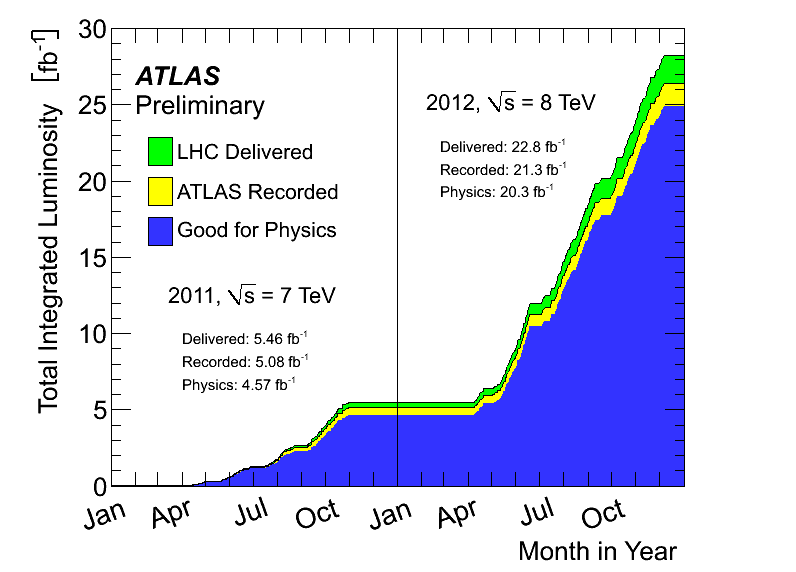
\includegraphics[width=0.5\textwidth]{Ch2/Img/LumiRun1.png}
    \caption{Cumulative luminosity versus time delivered to (green), recorded by ATLAS (yellow), and certified to be good quality data (blue) during stable beams and for pp collisions at 7 and 8 TeV centre-of-mass energy in 2011 and 2012 (Run 1).}
    \label{fig:chap2:LHC:Lumi:Run1}
\end{figure}
Figure \ref{fig:chap2:LHC:Lumi} shows the delivered and recorded luminosity during the Run 2 data taking \cite{Lumi2018}. $\mathcal{L}_{int} = 139$\ifb is used for physics since small fraction of full Run 2 data does not pass the good quality criteria compare to Run 1. For this reason the analyse described in this thesis is performed on the 2015-2018 data subsets.\\
\begin{figure}[ht]
    \centering
    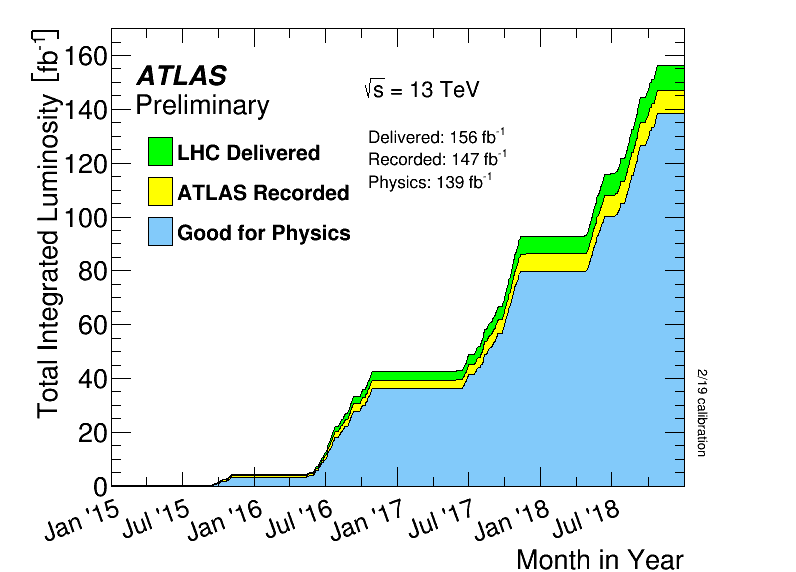
\includegraphics[width=0.6\textwidth]{Ch2/Img/Lumi.png}
    \caption{Luminosity delivered by the LHC during the Run 2 data taking. ATLAS recorded this data with an efficiency above 90\%.}
    \label{fig:chap2:LHC:Lumi}
\end{figure}
Knowing the cross section of the \HHyybb production, one can evaluate the number of events available for the analysis as $N_{HH\rightarrow\gamma\gamma\bar{b}b} = \mathcal{L}_{int}\cdot\sigma_{pp\rightarrow HH}\cdot Br(HH\rightarrow\gamma\gamma\bar{b}b)$ that leads to about 12 events.
\subsection{Pile-up}
\label{chap2:LHC:PU}
Because of the very high density of protons at the collision points, more than one proton interact when two LHC bunches cross each other at the center of the experiment. This is commonly referred to as pileup. On top of the usual $in-time$ pileup, defined as the collision events occurring during the same bunch-crossing as the event of interest, one also has to consider $out-of-time$ pileup, coming from remnants of information found in some of the detector subsystems that end-up being attributed to the wrong bunch-crossing, and therefore to the wrong event typically from previous collisions. Figure \ref{fig:chap2:LHC:PU} shows the average number of simultaneous interactions per bunch crossing for Run 2. \\
\begin{figure}[ht]
    \centering
    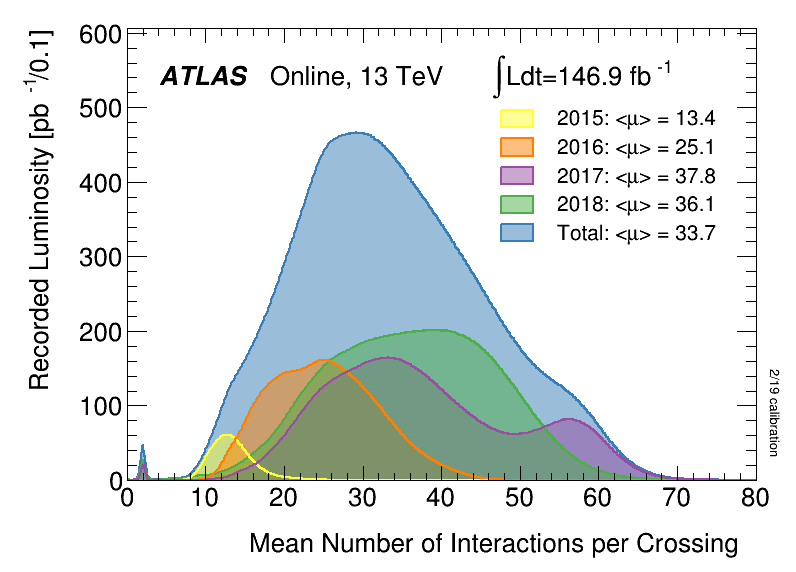
\includegraphics[width=0.6\textwidth]{Ch2/Img/PU.png}
    \caption{Recorded integrated luminosity as function of the mean number of interaction per bunch crossing in pp collisions recorded by the ATLAS detector during Run 2 at 13 TeV \cite{Lumi2018}.}
    \label{fig:chap2:LHC:PU}
\end{figure}

\section{ATLAS A Toroidal LHC ApparatuS detector}
\label{chap2:ATLAS}
The ATLAS detector is one of the four experiments placed on the four crossing points of the LHC beams. It is currently the largest experiment particle physics with a length of 46 m along the beam pipe and a transverse diameter of 25 m and more than 7000 tons of weight \cite{ATLAS_Exp}. It is a superposition of four sub-detectors, each optimized for the identification and the measurement of a specific category of particles : Inner Tracker, Electromagnetic Calorimeter (ECAL), Hadronic Calorimeter (HCAL) and Muons Spectrometer. It is composed of central called Barrel and two End-Cap to cover the $4\pi$ solid angle. Its geometry is optimised to detect particles produced orthogonal to the beam pipe and allow for forward detection to estimate the energy of invisible particles. The detector has been operating since 2008, taking alignment data with cosmic rays before the LHC launch, and its data is exploited by a collaboration of about 3000 scientific authors from 181 institutions in 38 countries. An overview sketch of the ATLAS detector is shown in Figure \ref{fig:chap2:ATLAS:Img}.
\begin{figure}[ht]
    \centering
    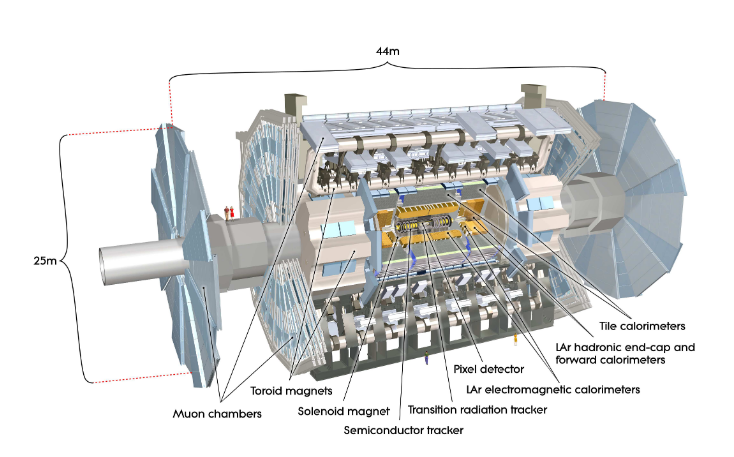
\includegraphics[width=0.8\textwidth]{Ch2/Img/ATLAS_sketch.png}
    \caption{Sketch of the ATLAS detector with its different sub-detectors.}
    \label{fig:chap2:ATLAS:Img}
\end{figure}

\subsection{Coordinated system}
\label{chap2:ATLAS:CS}
The coordinate system used in the ATLAS experiment is cylindrical coordinates where the z-axis is along the LHC beam pipe, the x-axis pointing toward the center of the LHC ring and the y-axis pointing upward. A physic object (particle) is identified by its transverse component of the three-momentum $p_T = \sqrt{p_X^2 + p_Y^2}$, its azimuthal angle $\phi \in [-\pi,\pi] $ formed by the three-momentum and the x-axis and its polar angle $\theta \in [0,\pi]$, i.e the angle between the three-momentum and the z-axis. \\
The polar angle is expressed in terms of the pseudo-rapidity $\eta$, defined as
\begin{equation}
\eta = -\log[\tan(\theta/2)].
\end{equation}
In collisions involving, the adoption of $\eta$ instead of $\theta$ ensure the detector balance over particles and particles distribution recorded is approximately flat with respect to $\eta$.
\begin{equation}
\frac{\partial\sigma_{QCD}}{\partial\eta} = cte.
\end{equation}
The pseudo-rapidity $\eta$ coincides for relativistic particles to the rapidity $y$, defined as 
\begin{equation}
y = \frac{1}{2}(\frac{E+p_Z}{E-p_Z}),
\end{equation}
where E is the particle energy.
Figure \ref{fig:chap2:ATLAS:SYS} shows the coordinate system common to ATLAS and CMS experiments.
\begin{figure}[ht]
    \centering
    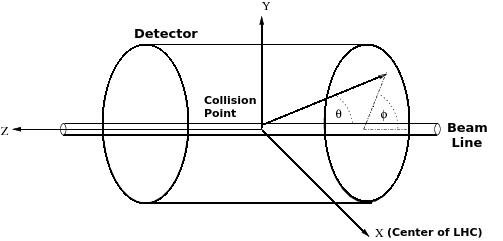
\includegraphics[width=0.6\textwidth]{Ch2/Img/ATLAS_Sys.jpeg}
    \caption{Coordinate system used by the ATLAS and CMS experiments at the LHC.}
    \label{fig:chap2:ATLAS:SYS}
\end{figure}

\subsection{The Inner Tracker}
\label{chap2:ATLAS:ITk}
The Inner Detector (ID) has been designed to detect and reconstruct the path of the electrically charged particle bent by a 2T solenoid magnetic field. It also provides a good momentum resolution by reconstructing the curvature and the direction, and both primary and secondary vertex measurements for tracks above approximately 0.5 GeV\cite{ID_TRD, TrkVertexing}. In terms of acceptance, the ID covers region of $|\eta|\leqslant2.5$. To achieve the momentum and vertex resolution requirements imposed by the physics goals at the LHC and the very large track density environment, the ID high-precision measurements must be made with fine detector granularity. The ID is composed of four complementary sub-detectors: IBL, the Pixel Detector, the Semi Conductor Tracker (SCT) and the Transition Radiation (TRT). The magnetic field of 2 T is provided by a solenoid inserted between the ID and the EM calorimeter. The layout of the Inner Detector (ID) is illustrated in Figure \ref{fig:chap2:ATLAS:ITK:ID}.
\begin{figure}[ht]
    \centering
    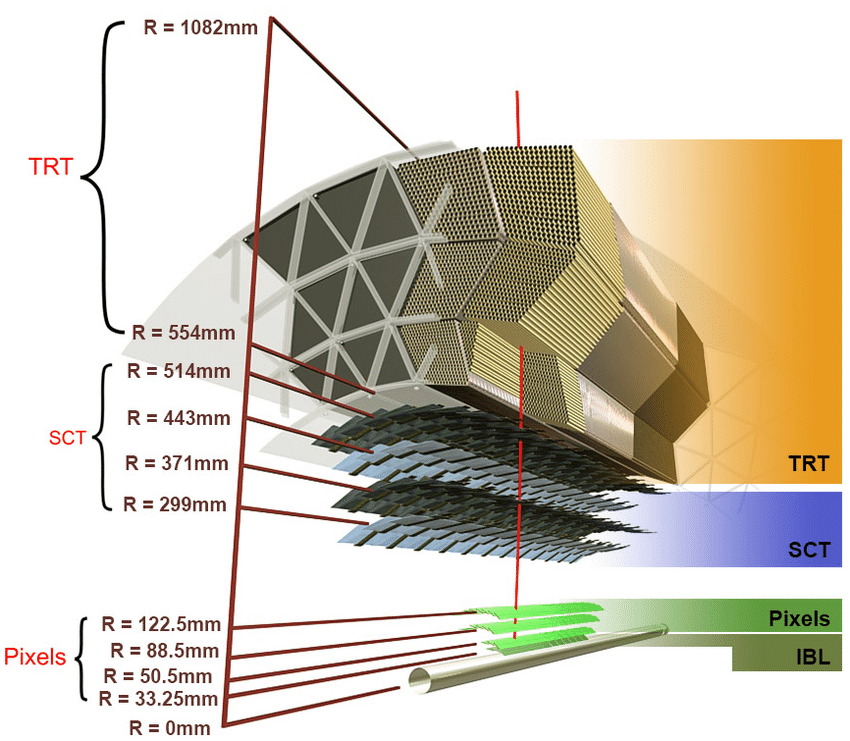
\includegraphics[width=0.5\textwidth]{Ch2/Img/ID_withIBL.png}
    \caption{Layout of the Inner Detector (ID) \cite{ID_withIBL}.}
    \label{fig:chap2:ATLAS:ITK:ID}
\end{figure}
\subsubsection{IBL}
\label{chap2:ATLAS:ITK:IBL}
In 2014, at the first LHC long shutdown, the ATLAS pixel detector was upgraded with a pixel layer installed close to the beam pipe called Insertable B-Layer (IBL) \cite{IBL_TDR}. Its motivations are :
\begin{itemize}
	\item Insure the good identification of the primary vertex which play an important role in $b$-jet identification ($b$-tagging), which in turn significantly improves the sensitivity of many analyses. Inefficiencies in the other layers can be partially compensated during reconstruction at the cost of an increased fake rate, the IBL restore the full $b$-tagging efficiency even in case of a complete B-layer failure.
	\item Luminosity effects, The current pixel detector was designed for a peak luminosity of $10^{34} cm^{-2}s^{-1}$. With high luminosity the event pileup is increased, leading to high occupancy that can induce readout inefficiencies, would thereby limit the $b$-tagging efficiency. The addition of the IBL layer helps to preserve tracking performance in face of luminosity effects.
\end{itemize}
Strong constraints and project specifications have a substantial impact on the technologies required for the IBL. IBL covers the region of $|\eta|< 2.58$ in pseudo-rapidity and located at a mean radius of 33.2 mm around the beam pipe. The pixels uses 12 million pixels with a typical size of 50x250 $\mu$m. The IBL consists of 14 staves with each 20 modules made using planar sensors. The temperature of the IBL is controlled using a bi-phase CO2 cooling system. Figure \ref{fig:chap2:ATLAS:ITK:IBL} shows the IBL within the Pixel Detector volume and around the beam pipe.
\begin{figure}[ht]
    \centering
    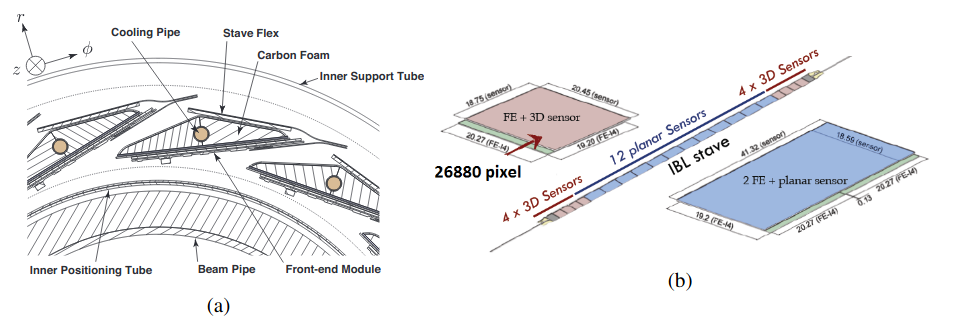
\includegraphics[width=0.8\textwidth]{Ch2/Img/IBL.png}
    \caption{(a) Transverse view of 3 of the Insertable-B-Layer (IBL) staves, located directly on the beam pipe. (b) The layout of one of the 14 IBL staves \cite{ID_withIBL}.}
    \label{fig:chap2:ATLAS:ITK:IBL}
\end{figure}

Additional measurement point provided by IBL improves significantly the reconstructed parameters by the tracker. Figure \ref{fig:chap2:ATLAS:ITK:IBL:Imp} shows the improvement in impact parameter resolution due to the IBL as measured from early Run 2 data with respect to Run 1. 
\begin{figure}[ht]
    \centering
    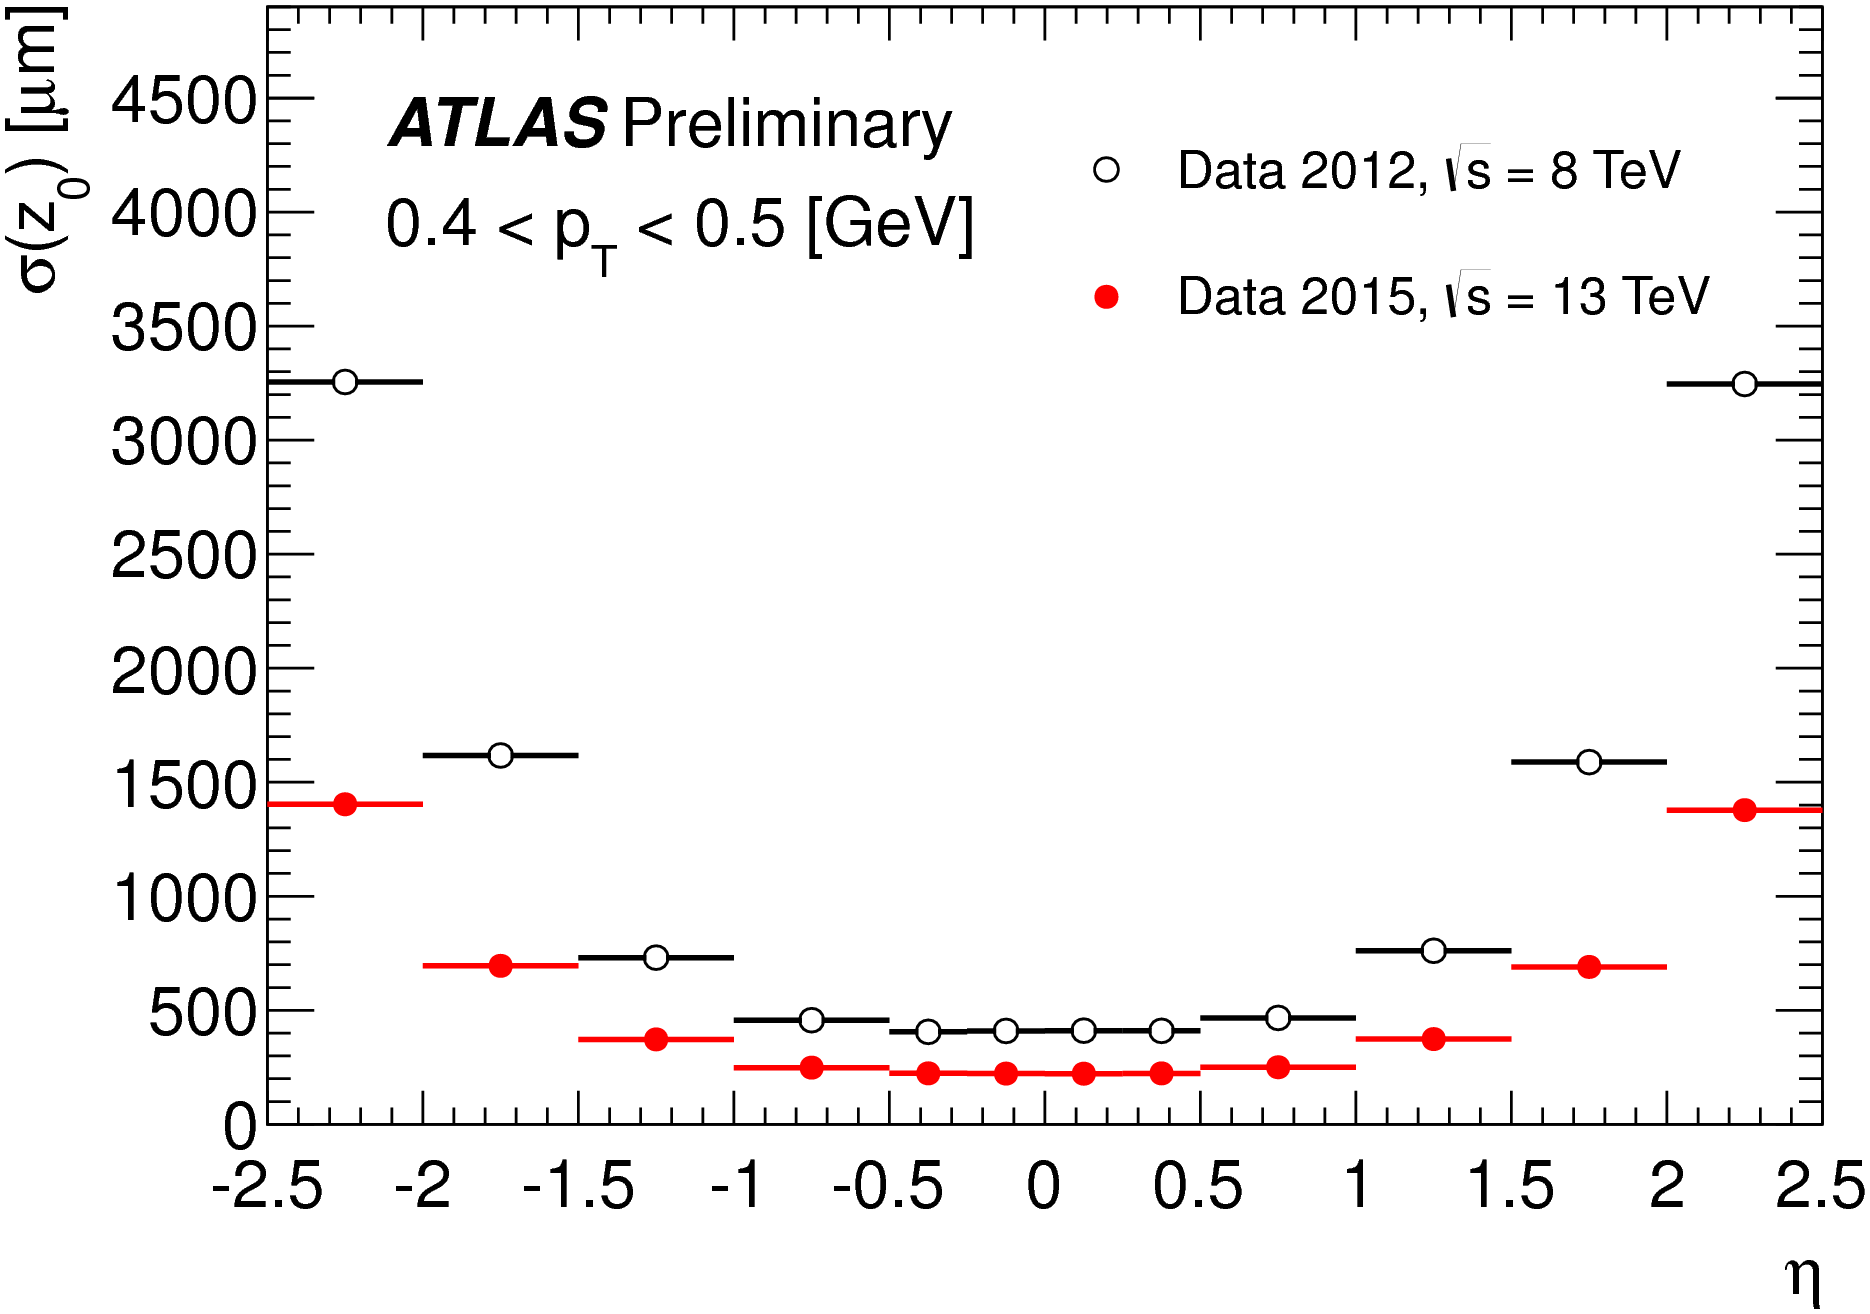
\includegraphics[width=0.6\textwidth]{Ch2/Img/IBL_impact.png}
    \caption{Unfolded longitudinal impact parameter resolution measured from data in 2015, $\sqrt{s}= 13$ TeV, with the Inner Detector including the IBL, as a function of $\eta$  for values of 0.4 < \pT < 0.5 GeV compared to that measured from data in 2012, $\sqrt{s} = 8$ TeV \cite{IBL_IP}.}
    \label{fig:chap2:ATLAS:ITK:IBL:Imp}
\end{figure}
In addition to a factor of 4 reduction in reconstruction times \cite{IBL_Time}, Figure \ref{fig:chap2:ATLAS:ITK:IBL:Trk} shows the improvement achieved with IBL for the performance of tracking in dense environments (TIDE). Improvements in tracking have a direct impact on vertex identification and $b$-tagging. 
\begin{figure}[ht]
    \centering
    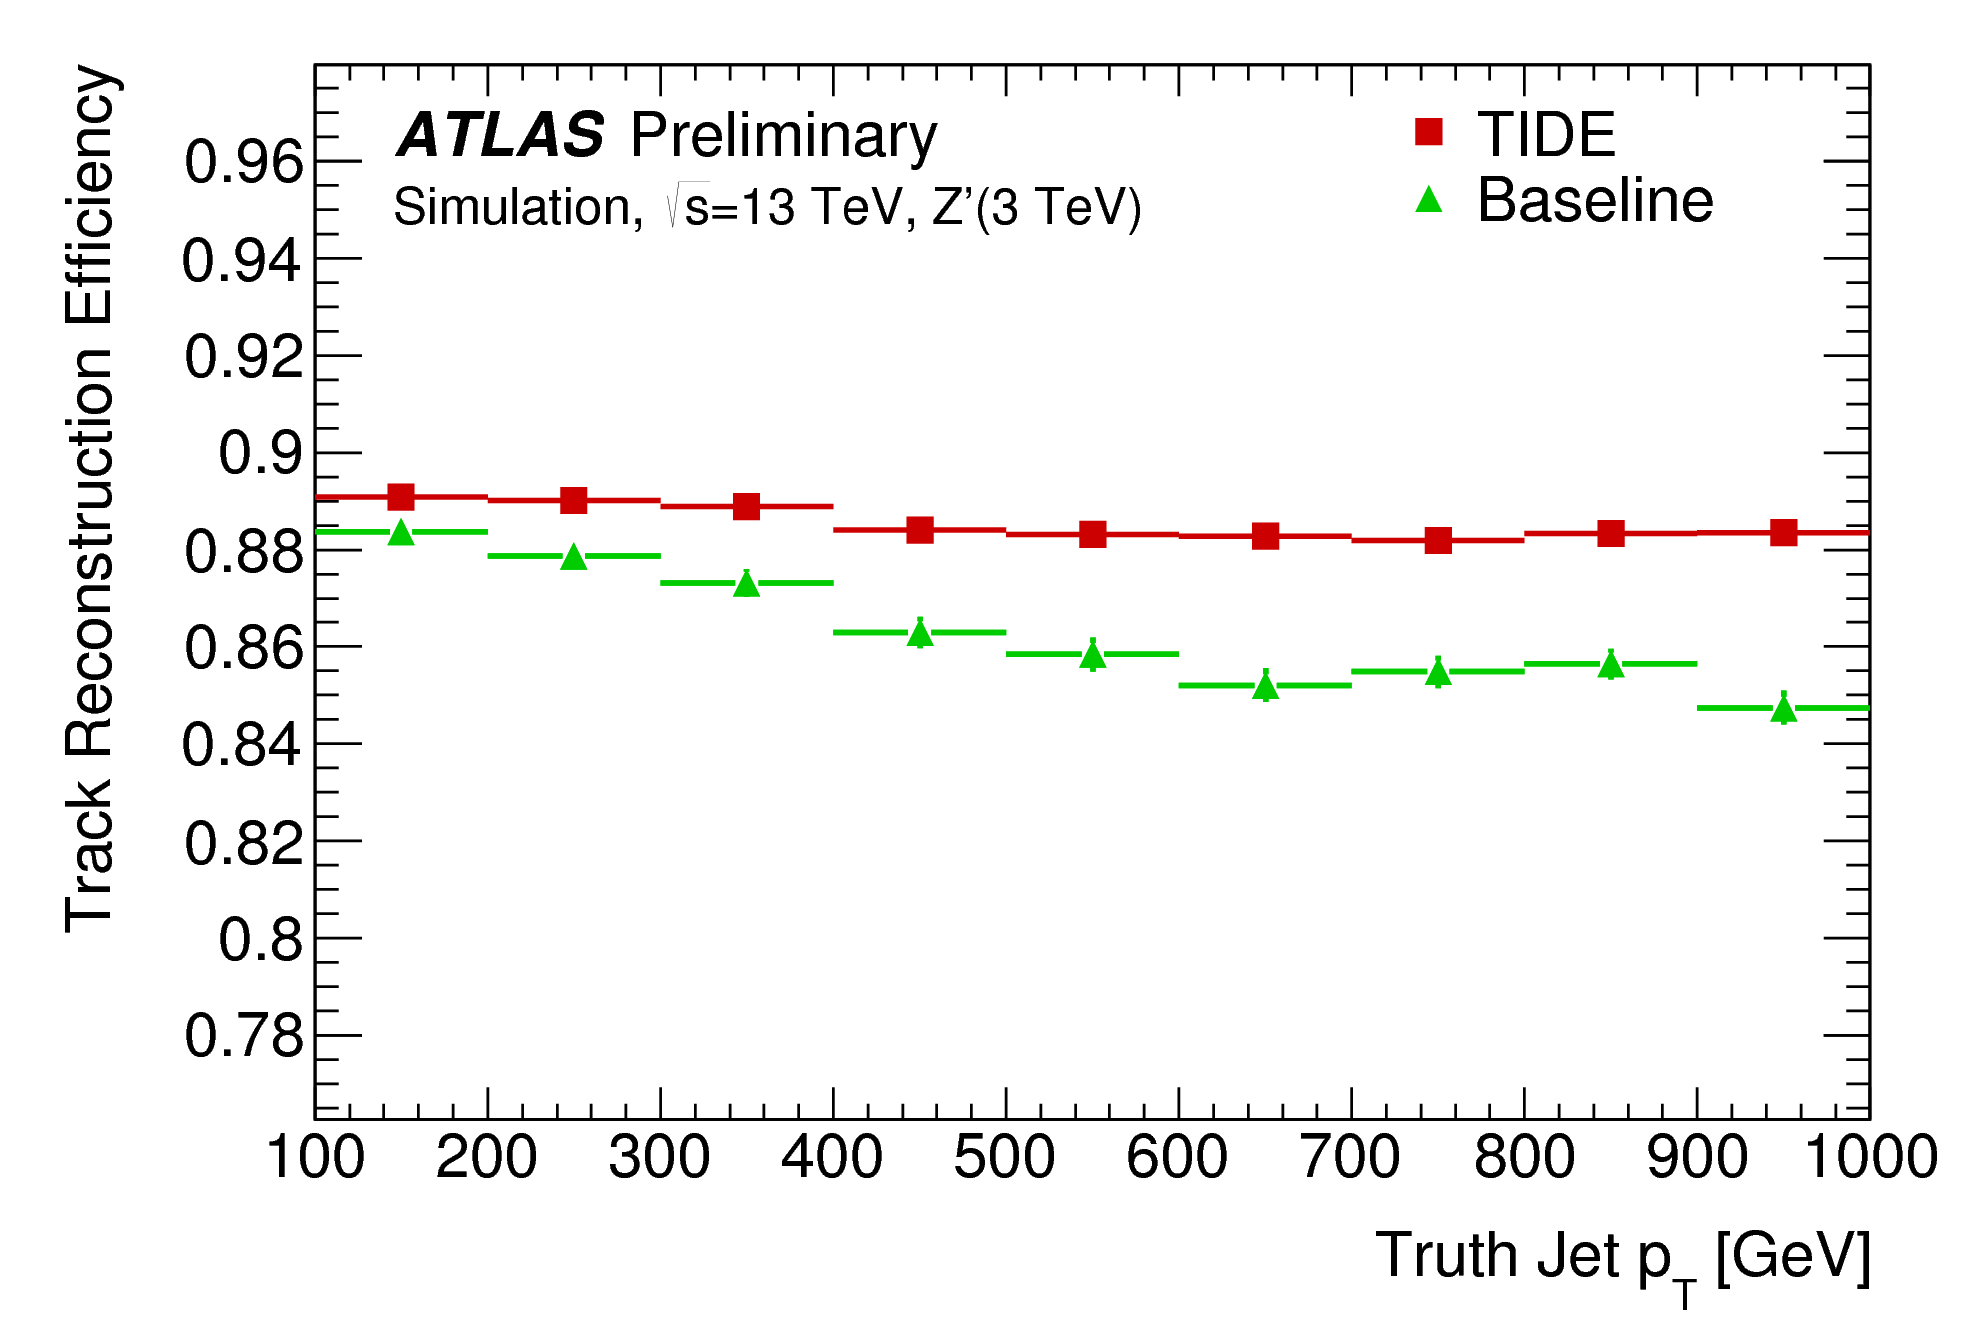
\includegraphics[width=0.6\textwidth]{Ch2/Img/IBL_track.png}
    \caption{The average efficiency to reconstruct primary tracks with a production vertex before the first layer in jets as a function of jet \pT. The same sample generation, with limited statistics, is used for both reconstruction algorithms resulting in correlated features \cite{IBL_Trk}.}
    \label{fig:chap2:ATLAS:ITK:IBL:Trk}
\end{figure}
Figure \ref{fig:chap2:ATLAS:ITK:IBL:Btag} shows the improvement in the $b$-tagging efficiency with IP3D+SV1 $b$-tagging algorithms respect to Run 1 algorithm due to the IBL \cite{IBL_Btag, IBL_Btag2}. The IP3D and SV1 algorithms will be explained later in the thesis.
\begin{figure}[ht]
    \centering
    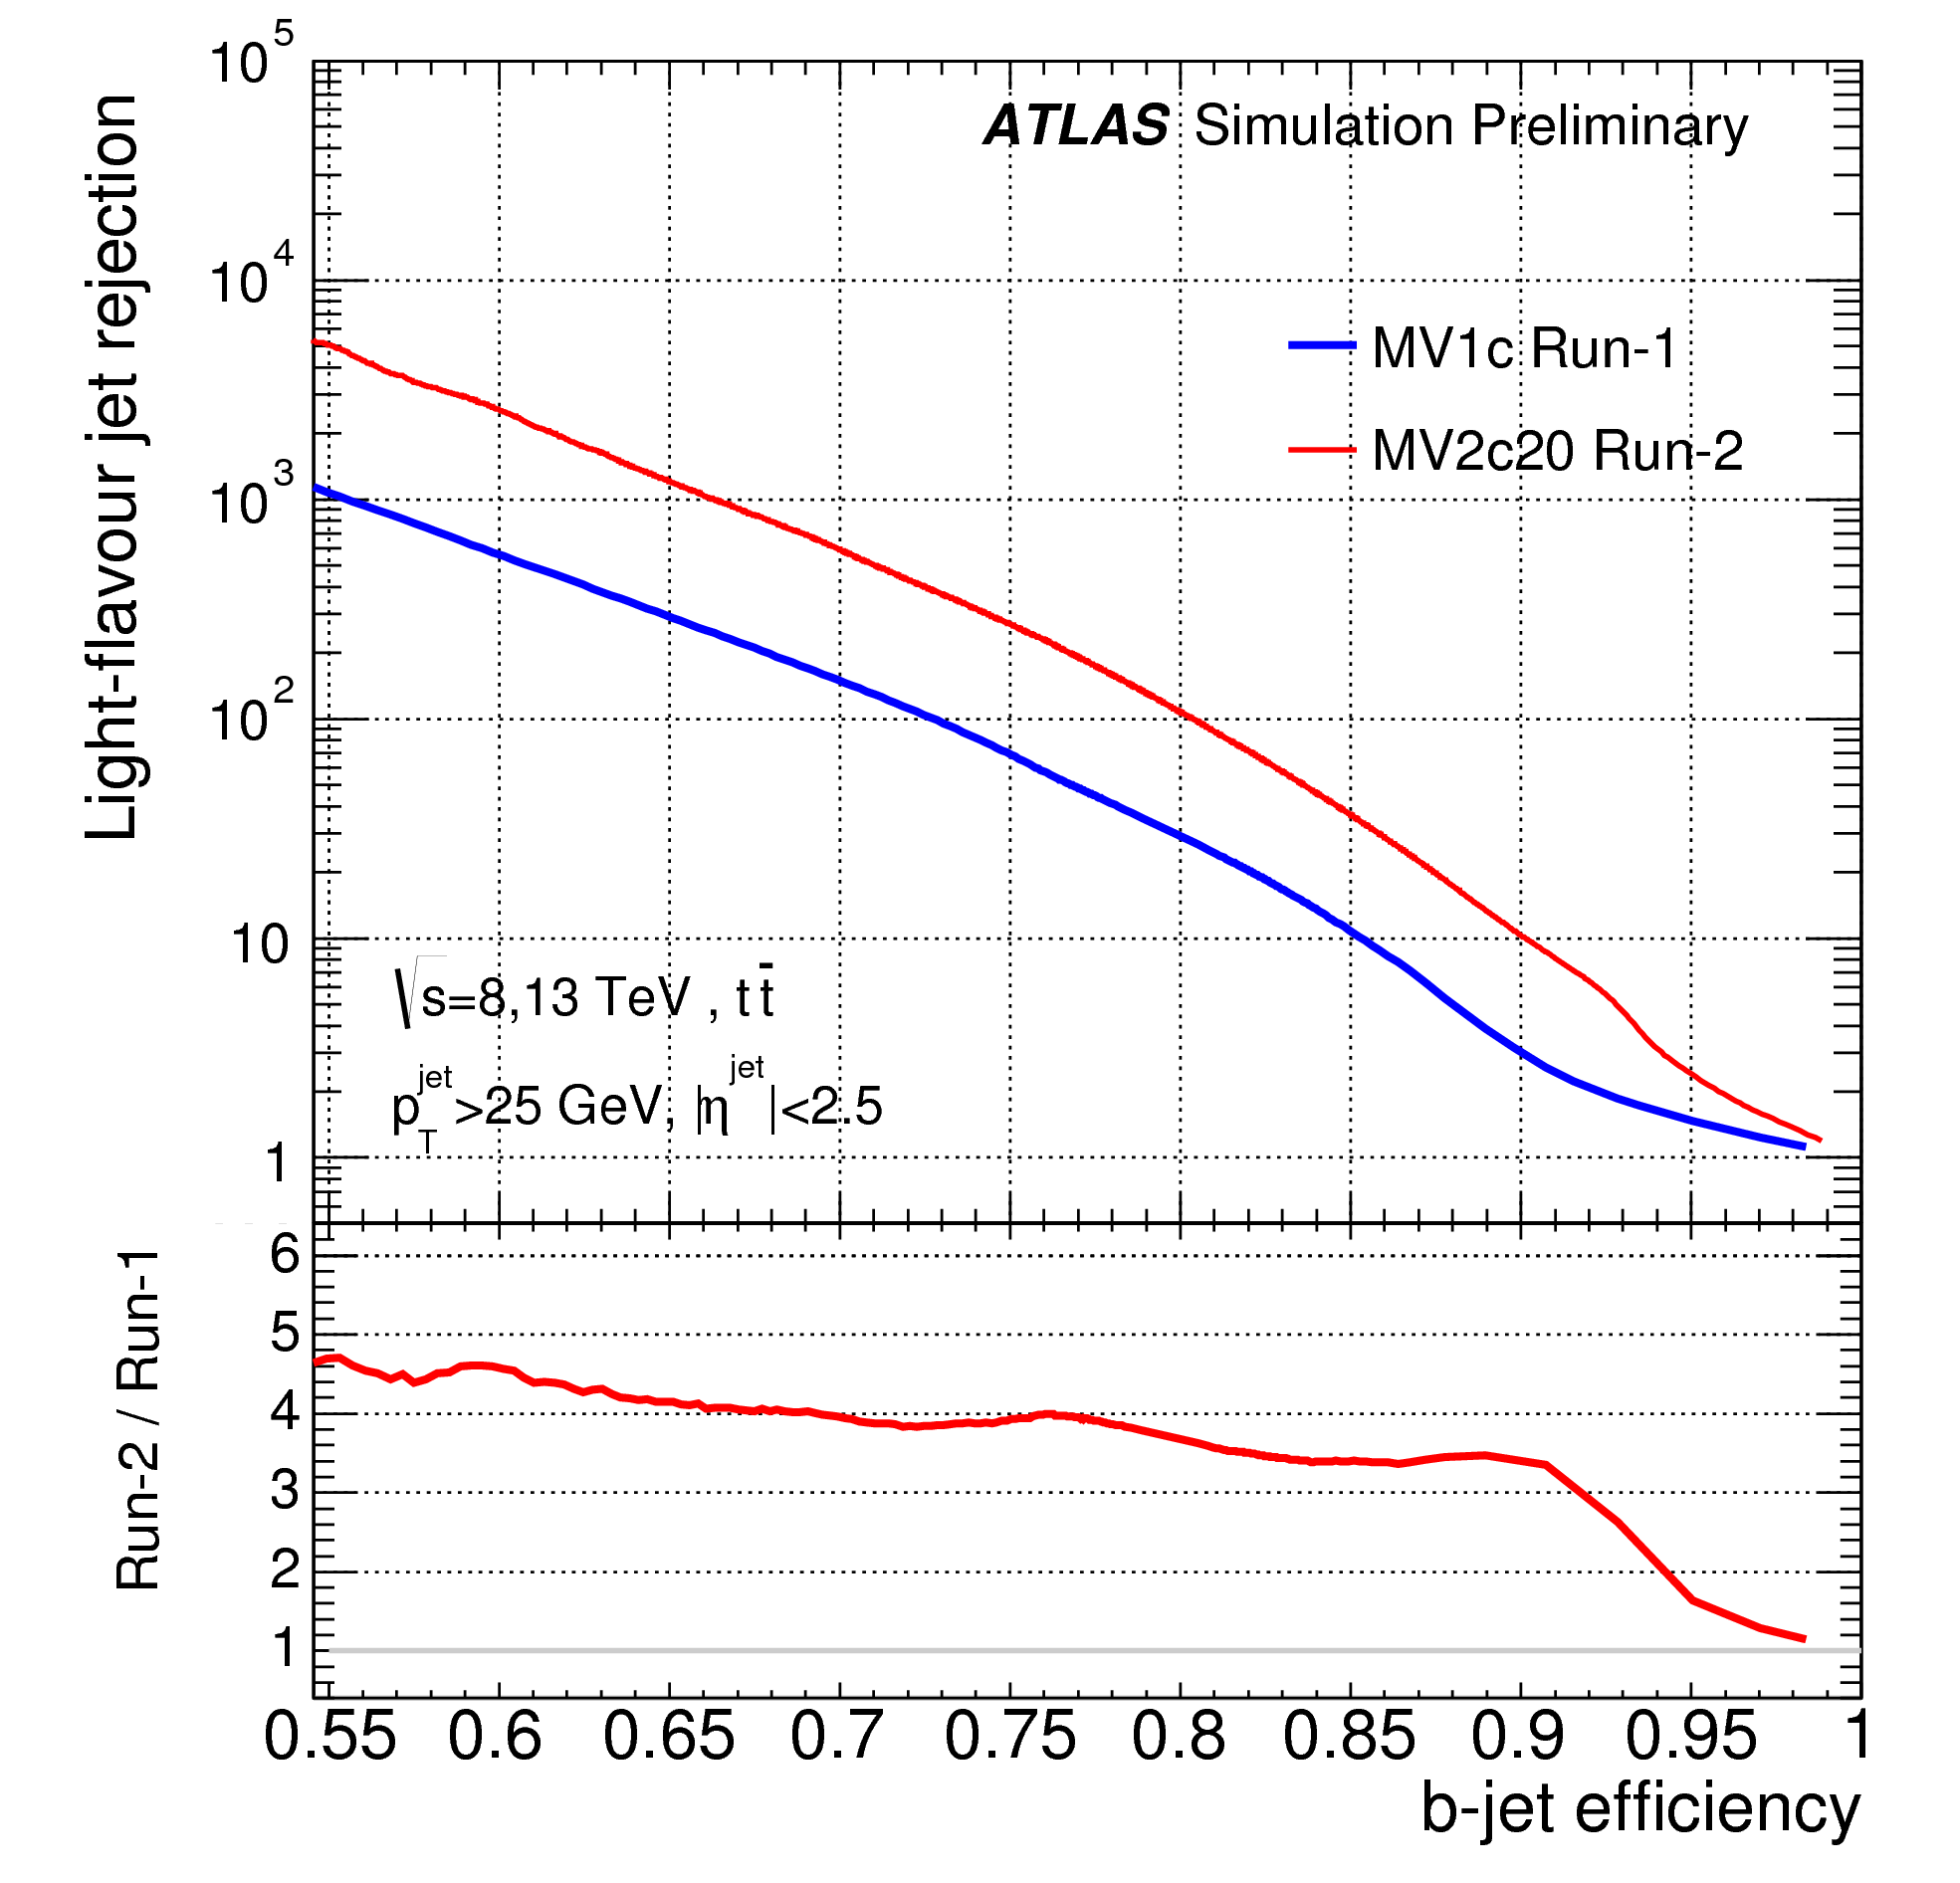
\includegraphics[width=0.6\textwidth]{Ch2/Img/IBL_btag2.png}
    \caption{Rejection factor against light jets as a function of $b$-jet efficiency for t the combined IP3D+SV1 tagger. Compared are the results with and without IBL.}
    \label{fig:chap2:ATLAS:ITK:IBL:Btag}
\end{figure}
\subsubsection{Pixel Detector}
\label{chap2:ATLAS:ITK:PD}
With the existing technology at that time (2000s), the Pixel Detector (PD) is designed to provide high-granularity, high-precision measurements as close as possible to the interaction point (IP). It consists of three barrel layers placed at the radius of 50.5 mm , 88.5 mm and 122.5 mm centered around the beam axis and two end-cap with three disc layers each positioned at $|z|= 495.580$ and $650 \ mm$. It provides three measurement points per track. The system is designed to be highly modular, containing approximately 1500 identical barrel modules and 1000 identical disk modules, each module is composed of 61440 pixel elements of silicon semi-conductor. In total there are about 80 million readout channels in the whole PD. The spatial resolution for the barrel modules is 10 $\mu$m in r-$\phi$ and 66 $\mu$m in z, for the end-caps the spatial resolution in r-$\phi$ is same as the barrel and 115$\mu$m in r. The main limitation of the pixel detector is the radiation hardness as the expected fluence is at the tolerable limit. 
\subsubsection{Semi Conductor Tracker}
\label{chap2:ATLAS:ITK:SCT}
The SCT system is designed to provide four precision points per track in the intermediate radial range, contributing to the measurement of momentum, impact parameter and vertex position. The barrel and end-caps SCT are four layers of silicon microstrip for barrel and nine disks for end-caps. The spatial resolution is 16 $\mu$m in r-$\phi$ for both the barrel and the end-caps. The four complete barrels are positioned in radius of 300, 373, 447 and 520 mm. Tracks can be distinguished if separated by more than $\sim$200 $\mu$m. There are 6.3 millions readout channels for the SCT.
\subsubsection{Transition Radiation Tracker}
The TRT is positioned at the outer part of the ID. It consist of 370000 drift tubes called straws. Each straw has a diameter of 4 mm and 1.44 m in long. The straws are filled with a gas mixture of 70\% $Xe$, 27\% $CO_2$ and 3\% $O_2$. Its wall acts as a cathode and kept at high voltage. The anode is a 30 $\mu$m diameter plated tungsten wire placed in the center of the straw. When a charged particle traverses a straw, it ionizes the gas and the produced electrons travel through the anode generating an electric signal. To keep the TRT performance to be constant, the close-loop gas system is used maintaining the correct gas fractions. The straws are arranged to be parallel to the beam-pipe in the barrel and perpendicular in the end-cap region. There are about 50k straws in the barrel and 320k straws in the end-cap providing high precision measurement for each track. The radial resolution is about 130 $\mu m$. \\
In the Perigee representation, tracks are described using the parameters of a helical trajectory at the point of closest approach to the z-axis: the transverse impact parameter $d_0$, the z coordinate $z_0$, the angles $\theta$ and $\phi$ and the inverse of the particle momentum multiplied by the charge q/p, as illustrated in Figure \ref{fig:chap2:ATLAS:ITK:Trk}
\begin{figure}[ht]
    \centering
    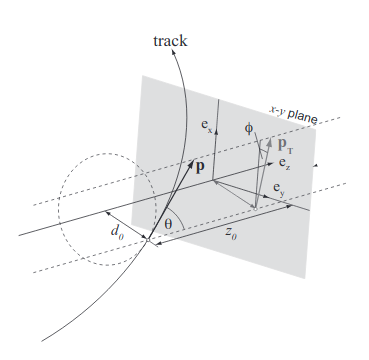
\includegraphics[width=0.5\textwidth]{Ch2/Img/Track.png}
    \caption{The Perigee representation of the track \cite{Track_schema}.}
    \label{fig:chap2:ATLAS:ITK:Trk}
\end{figure}
The expected momentum resolution of the inner detector, without the IBL, is given by:
\begin{equation}
    \sigma(1/p_T)\cdot p_T = 0.036\%\cdot p_T [GeV] \oplus 1.3\%,
\end{equation}
$\oplus$ denote the quadrature addition.
\subsection{Calorimeter system}
\label{chap2:ATLAS:Calo}

Based on the calorimetry, the ATLAS calorimeter system is designed to provide a precise energy and position reconstruction for electromagnetic particles (electrons, photons) and jets (hadrons). The good hermiticity of the calorimeter ($|\eta|$ up to 5) also allows to measure the missing transverse energy and provides the separation of electrons and photons from hadrons and jets. The calorimeter system is composed of two calorimeters: the electromagnetic calorimeter (ECal) and the hadronic calorimeter (HCal). Both are sampling calorimeters, with alternating layers of a heavy absorber material and an active material in which an ionisation signal is produced. Figure \ref{fig:chap2:ATLAS:Calo} shows a three dimensional view of the ATLAS calorimeter system.
\begin{figure}[ht]
    \centering
    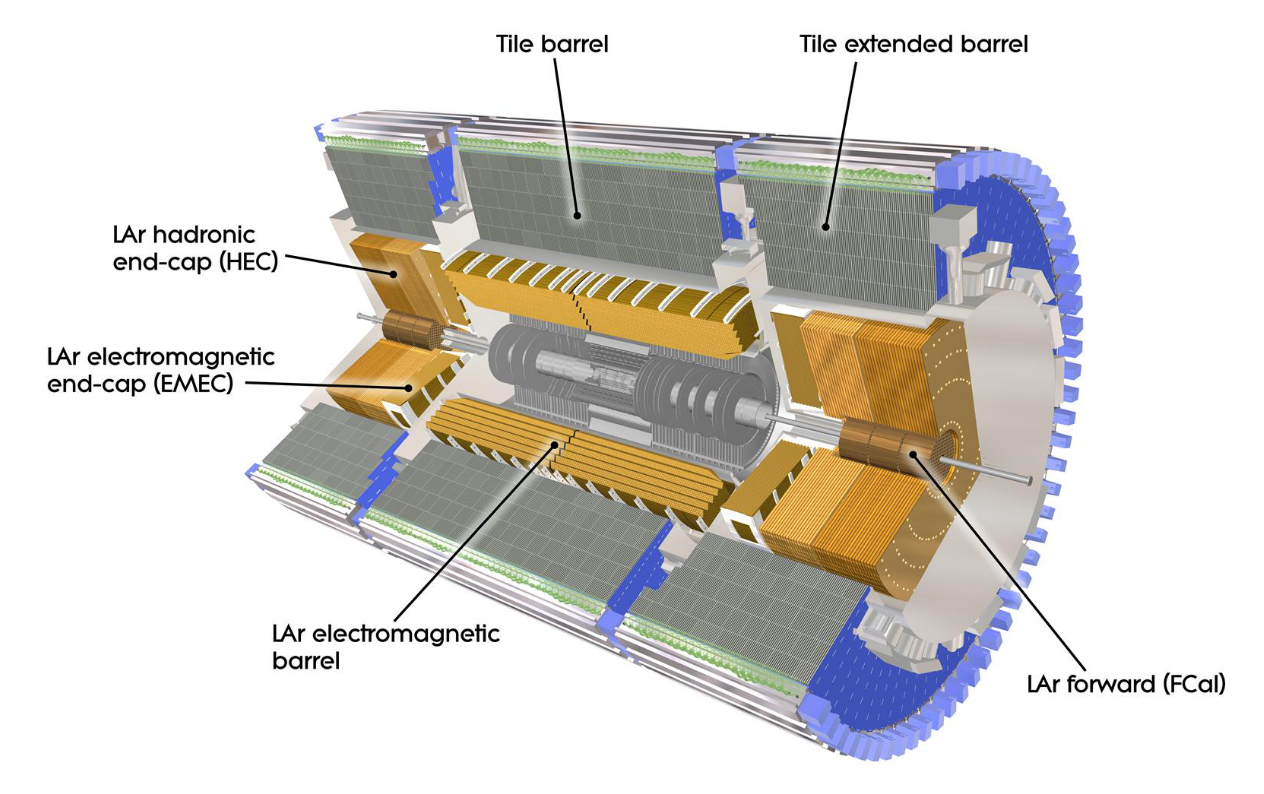
\includegraphics[width=0.6\textwidth]{Ch2/Img/Calo.png}
    \caption{ATLAS Calorimeter system.}
    \label{fig:chap2:ATLAS:Calo}
\end{figure}

\subsubsection{Electromagnetic calorimeter}
\label{chap2:ATLAS:Calo:ECAL}
The ECal is the first sub-detector after the ID. Is optimised for the reconstruction of the energy of electrons and photons exploiting their showers \cite{LAr_TRD}. It covers the region of $|\eta|<$3.2 excluding the region 1.375 $<|\eta|<$ 1.52 which correspond to the transition region between the barrel and end-caps. The barrel part covers $|\eta|<$1.475, while the two end-caps cover 1.375$<|\eta|<$3.2. The barrel and end-caps are composed of alternated layers of absorbing material lead (Z=82) ead plates ($\sim$1 mm thick), to enforce the development of the full EM showers within EM envelop and separated by active medium Liquid Argon (LAr) of 2 mm thick. The advantages of LAr, such as radiation hardness, intrinsic linear behaviour, cheapness compared to other noble gases, have been considered to outweigh the difficulties associated with the need of cryostats and signal feed-throughs. The total thickness of the calorimeter is at least 22 radiation lengths in the barrel, and more than 24 radiation lengths in the end-caps. The radiation lengths $X_0$ is defined as the scale after which high-energy electrons loose all but 1/e of their initial energy. $X_0$ of lead is 5.6mm. \\
Electrons and photons traversing the calorimeters initiate electromagnetic cascades, in which $e^+e^-$ pair production and bremsstrahlung processes occur. High-energy electrons predominantly loose energy in matter through bremsstrahlung, while high-energy photons create $e^+e^-$. EM particle produce shower when passed through ECal until its energy falls below the critical energy $E_c$. $E_c$, can be defined as the energy for which the energy loss per $X_0$ due to ionisation of the material is equal to the particle energy. In lead, $E_c$=7.4 MeV for electrons. The EM shower ionizes the atom of the liquid Argon generating an electric signal proportional to the energy deposit by the particle. The ionization is drifted to the electrode under electric field generated by the high voltage of 2000 V. To provide a huge signal response and hermiticity, ATLAS Collaboration adopted a particular geometry for the ECal: $accordion$ geometry. In the barrel, the accordion waves are axial and run in $\phi$; the folding angles of the waves vary with radius to keep the liquid-argon gap constant and reduce the died zone. In the end-caps, the waves are parallel to the radial direction and run axially. The size of the drift gap on each side of the electrode is 2.1 mm. Figure \ref{fig:chap2:ATLAS:Calo:ECal:Acc} shows the accordion shape of the EM calorimeter.
\begin{figure}[ht]
    \centering
    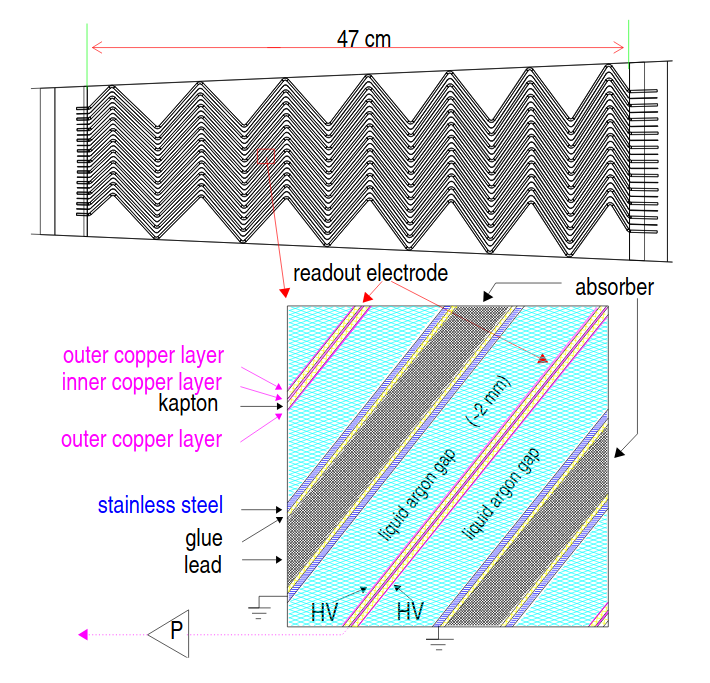
\includegraphics[width=0.6\textwidth]{Ch2/Img/ECal_accord.png}
    \caption{Accordion shape of the EM calorimeter.}
    \label{fig:chap2:ATLAS:Calo:ECal:Acc}
\end{figure}
The ECal is further segmented in three longitudinal layers, to measure the longitudinal shower development called respectively strip, middle and back. It has different EM cells granularity $\Delta\eta\times\Delta\phi$ per layer. Cells of the middle layer (Lr2) in the barrel region are $0.025\times0.025$, while for the strip (Lr1) cells are 8 times finer in the $|\eta|$ direction providing a precise $\eta$ measurement of incident particles. The back layer (Lr3) cells has a twice coarser granularity in $\eta$ and the same $\phi$ segmentation as in Lr2. Before the EM barrel calorimeter there is a Presampler (PS) LAr detector (Lr0), covering range $|\eta|<$1.8 and placed placed to start the shower before the calorimeter. PS has the finest granularity with a cell size of $\Delta\eta\times\Delta\phi = 0.003\times0.1$ used for $\pi\rightarrow\gamma\gamma$ background separation. The number of samplings  and the granularity in each of the samplings are summarized in Table \ref{tab:chap2:ATLAS:Calo:ECal:Gr}.
\begin{table}[ht]
    \centering
    \begin{tabular}{cccccc}
    \hline
    Sampling & $|\eta|<$1.5 & 1.5$<|\eta|<$1.8 & 1.8$<|\eta|<$2.0 & 2.0$<|\eta|<$2.5 & 2.5$<|\eta|<$3.2 \\
    \hline
    \hline
        Presampling & 0.025$\times$0.1 & 0.025$\times$0.1  \\
        Strip & 0.025/8$\times$0.1 & 0.025/8$\times$0.1 & 0.025/6$\times$0.1 & 0.025/4$\times$0.1 & 0.1$\times$0.1 \\
        Middle & 0.025$\times$0.025 & 0.025$\times$0.025 & 0.025$\times$0.025 & 0.025$\times$0.025 & 0.1$\times$0.1 \\
        Back & 0.050$\times$0.025 & 0.05$\times$0.025 & 0.05$\times$0.025 & 0.05$\times$0.025 \\
        \hline
    \end{tabular}
    \caption{Granularity of the EM calorimeter ($\Delta\eta\times\Delta\phi$) \cite{LAr_TRD}.}
    \label{tab:chap2:ATLAS:Calo:ECal:Gr}
\end{table}
Physics studies showed that precision physics can hardly be extended beyond a pseudorapidity of 2.5. For this reason, the small wheel has a coarser granularity and only two samplings in depth. EM calorimeter resolution is given by:
\begin{equation}
    \sigma_E/E = \frac{10\%}{E} \oplus 0.17\%.
\end{equation}
\subsubsection{Hadronic calorimeter}
\label{chap2:ATLAS:Calo:HCAL}
 At high energy colliders, quarks and gluons fragment to a beam of particles called jets (hadronic showering). The Hadronic Calorimeter (HCal) completes the measurement of the jets energy \cite{Tile_TDR}. Hadronic showers are larger than electromagnetic ones, thus it needs to be large enough to contain the hadronic showers and reduce the punch-through hadrons penetrating to the muon system. The total thickness is chosen to be about 11 $X_0$ to allows to have good performance on resolution for high energy jets. The hadronic calorimeter is divided into the Tile calorimeter and the LAr hadronic end-caps calorimeter. The barrel calorimeter is made of steel as absorbing material and scintillating plastic tiles as active medium and cover the range $|\eta|<1$ with two extensions in the range 0.8$<|\eta|<$1.7. The end-caps cover the range 1.5$<|\eta|<$3.2 and it is composed of two wheels made of parallel copper plates with LAr as active material in between. For the determination of the missing energy a good hermetic coverage is essential. Therefore ATLAS calorimeter is also equipped with a calorimeter covering the very forward region of 3.1$<|\eta|<$4.9 the LAr Forward Calorimeter (FCal). \\
 \textbf{The Tile} calorimeter provides signal by the tiles scintillation. The tiles are perpendicular to the beam-pipe with 3 mm thick. It is consists of a barrel ($|\eta|<$1.0) and two extended barrels (0.8$<|\eta|<$1.7). The Tile calorimeter is segmented into three layers. The dimension of the cells corresponds to $\Delta\eta\times\Delta\phi= 0.1\times0.1$ in first two layers and $\Delta\eta\times\Delta\phi= 0.2\times0.1$ in the last layer to contain the hadronic shower. A vertical gap of 68 cm wide between the barrel and extended barrel regions is used for passage of cables from the ID and the EM calorimeter. \\
 \textbf{LAr} cover end-cap and forward regions with 1.5$<|\eta|<$4.9. Each end-cap calorimeter (HEC) consists of two independent wheels of equal diameter with copper absorber plates. The end-cap calorimeter is divided into front, middle and back longitudinal layers. The FCal is placed at a distance of about 5 meters from the interaction point. It high density detector facing a very high particle flux and consisting of three wheels on each side employing liquid argon as an active material. The innermost wheel is optimized for electromagnetic showers and employs copper as the absorber. While the other two wheels measure hadronic showers using tungsten as absorbing material. The granularity of the hadronic LAr calorimeter is $\Delta\eta\times\Delta\phi= 0.1\times0.1$ for 1.5$<|\eta|<$2.5 and $\Delta\eta\times\Delta\phi= 0.2\times0.2$ for 2.5$<|\eta|<$3.2 while the forward calorimeter has $\Delta\eta\times\Delta\phi= 0.2\times0.2$. 
 %The forward calorimeters are also capable to reconstruct electrons. 
 The HCal is designed to measure the energy with a resolution of \cite{Tile_Perf}:
 \begin{equation}
     \sigma_E/E = \frac{50\%}{E} \oplus 3\%.
 \end{equation}

\subsection{Muon Spectrometer}
\label{chap2:ATLAS:MS}
Muons are minimally ionising particles in the detector due to their relatively high mass, therefore are not stopped by the calorimeter. The Muon Spectrometer (MS) is the outermost part of the ATLAS detector dedicated to detect muons exiting the calorimeter and measure their momentum in the range of $|\eta| < 2.7$ \cite{Muon_TDR}. A large superconducting air-cored toroid magnet is used to bend muons trajectories. Over the range $|\eta| < 1.4$, magnetic bending is provided by the large barrel toroid. For $1.6<|\eta| < 2.7$ region muon tracks are bent by two smaller end-cap magnets inserted into both ends of the barrel toroid. Over $1.4<|\eta|<1.6$, usually referred to as the transition region, magnetic deflection is provided by a combination of barrel and end-cap fields. Two different functions are accomplished by the MS: triggering and high precision tracking. The tracking is performed by the Monitored Drift Tubes (MDTs) and by Cathod Strips Chambers (CSCs) at large pseudo-rapidity. However, trigger system covers the region up to $|\eta| < 2.4$, and it is composed by Resistive Plate Chambers (RPCs) in the barrel and Thin Gap Chamber (TGC) in the end-caps. The conceptual layout of the spectrometeris shown in Figures \ref{fig:chap2:ATLAS:MS}. \\
\begin{figure}[ht]
    \centering
    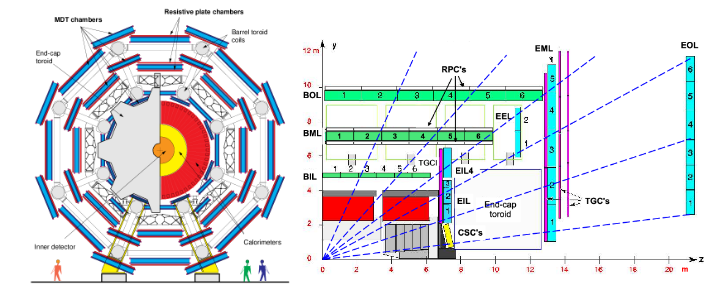
\includegraphics[width=0.75\textwidth]{Ch2/Img/Muon.png}
    \caption{Side view of one quadrant ($right$) and transverse view ($left$) of the muon spectrometer.}
    \label{fig:chap2:ATLAS:MS}
\end{figure}
The Monitored Drift Tubes are aluminium drift tubes with a diameter of 29.970 mm as Figure \ref{fig:chap2:ATLAS:MS:Tube} shows, operating with a gas mixture of 93\% of $Ar$ and 7\% of $CO_2$ Ar/CO2 at 3 bar pressure. Each chamber consists of two sections with three (inner station) or four (middle and outer station) layers of the drift tubes. Tungsten-rhenium wire of 50$\mu$m collects the electrons resulting from ionization at a potential of 3 kV. The maximum drift time can reach about 700 ns. The MDTs are designed for precise tracking of muons and cover most of the MS pseudorapidity total coverage, with a single-hit resolution of about 35 $\mu$m per chamber. \\
\begin{figure}[ht]
    \centering
    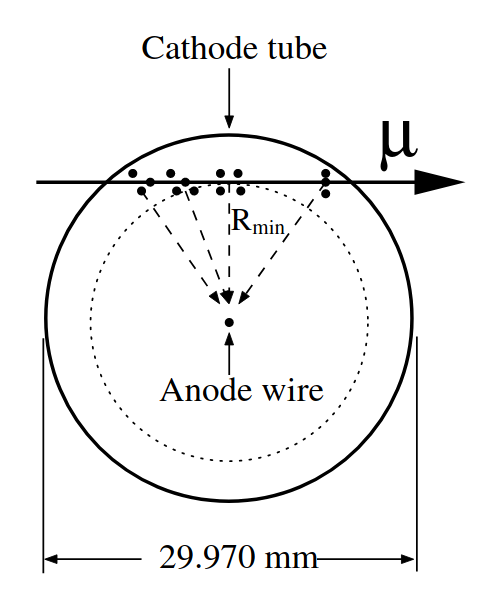
\includegraphics[width=0.35\textwidth]{Ch2/Img/Tube.png}
    \caption{Transverse cross section of the MDT tube.}
    \label{fig:chap2:ATLAS:MS:Tube}
\end{figure}
The Cathode-Strip Chambers are multi-wire proportional chambers filled with a mixture of 80\% of $Ar$ and 20\% of $CO_2$ with cathode planes segmented into strips in an orthogonal direction to the beam axis. The CSCs cover the range of 2.0$<|\eta|<$2.7 which is partially covered by the ID and has higher particle flux, because of their better time resolution and rate capability than MDTs. The CSC chambers have a slightly lower resolution than the MDTs, with 40 $\mu$m in the tracks bending plane, and 5 mm in the transverse plane. \\
For trigger purpose, the RPCs placed in the barrel, covering the range $|\eta|<$1.05,  are arranged into three concentric layers around the beam axis and placed before or after the MDT layers as Figure shows \ref{fig:chap2:ATLAS:MS}. The RPC unit is composed of gap of 2 mm formed  by two parallel electrodes. The gap is filled with a mixture gas of 94.7\% of $C_2H_2F_4$, 5\% of $Iso-C_2H_2F_4$ and 0.3\% of $SF_6$ $C_2H_2F_4$. The electric field between electrodes is about 4.9 kV/mm. The end-caps are equipped with the TGCs up to $|\eta|=$ 2.4.The TGCs are multi-wire proportional chambers filled with a mixture 55\% of $CO_2$ and 45\% of $n-C_5H_{12}$. The TGCs are arranged in
seven layers in each side.\\
The overall momentum resolution $\frac{\sigma_{p_T}}{p_T}$ provided by the muon system is 4\% (1\%) at 5GeV (1TeV) \cite{ATLAS_Perf}.

\subsection{Trigger}
\label{chap2:ATLAS:Trigger}
Collision rate at the center of ATLAS is 40MHz due to the bunch crossing in each 25 ns provided by LHC. At such a rate, it is technically not possible to fully process and store all data recorded by the ATLAS detector. The ATLAS trigger system was design to handle this problem, the purpose of the trigger system is to reduce the input of 40 MHz bunch crossing rate to an output rate of about 200 Hz in order to record them for further analysis. This is done thanks to two separated trigger systems. The first level so-called Level-1 (L1) \cite{Trigger_L1} is a hardware-based trigger that uses reduced granularity signals from the calorimeter and the muon spectrometer to identify Regions-Of-Interest (ROI) with high energy objects or high multiplicity at a latency of 2.5 $\mu$s. The L1 trigger system is responsible for reducing the rate to at least 75 kHz. Events passing the L1 trigger are then sent to the software-based High-Level Trigger (HLT) \cite{Trigger_HLT}. At the HLT, a fast analysis of these ROTs followed by an offline-like reconstruction of the events takes place with a processing time of around 0.2 s. The HLT creates output with a frequency of around 1 kHz. Often the final output rate cannot be made small enough \cite{DQ}. In this case only random events are selected and stored.
\section{Physics objects reconstruction}
\label{chap2:Objects}
ATLAS provides energy deposits collected by sub-detectors. To interpret this raw output in terms of the event particles an advanced particle reconstruction chains have to be employed. These are described in this Section.

\subsection{Track and Vertex reconstruction}
\label{chap2:Objects:Trk}
Tracks are reconstructed in the ID (Section \ref{chap2:ATLAS:ITk}) using a sequence of algorithms \cite{Track_Reco, New_Trk}. The inside-out algorithm starts from three points seeds in the SCT.  A combinatorial Kalman filter (Iterative algorithm that provides best estimate of the state based on projection of earlier measurements and current measurement \cite{Kalman} ) is then used to build track candidates from the chosen seeds by incorporating additional space-points from the remaining layers of the pixel and SCT detectors which are compatible with the preliminary trajectory. Ambiguities in the track candidates are resolved, and tracks are extended into the TRT. The inside-out algorithm is the baseline algorithm designed for the efficient reconstruction of primary charged particles. In a second stage, a back-tracking algorithm is used in track search starting from segments reconstructed in the TRT and extending them inwards by adding silicon hits. The back-tracking is designed to reconstruct secondaries particles. Finally tracks with a TRT segment but no extension into the silicon detectors are referred as TRT-standalone tracks. The track reconstruction efficiency is defined as the fraction of primary particles with \pT $>$ 400 MeV and $|\eta|<$ 2.5 matched to a reconstructed track. Figure \ref{fig:chap2:Objects:Trk:Eff} shows the track reconstruction efficiency as a function of \pT and $\eta$.
\begin{figure}[ht]
    \centering
    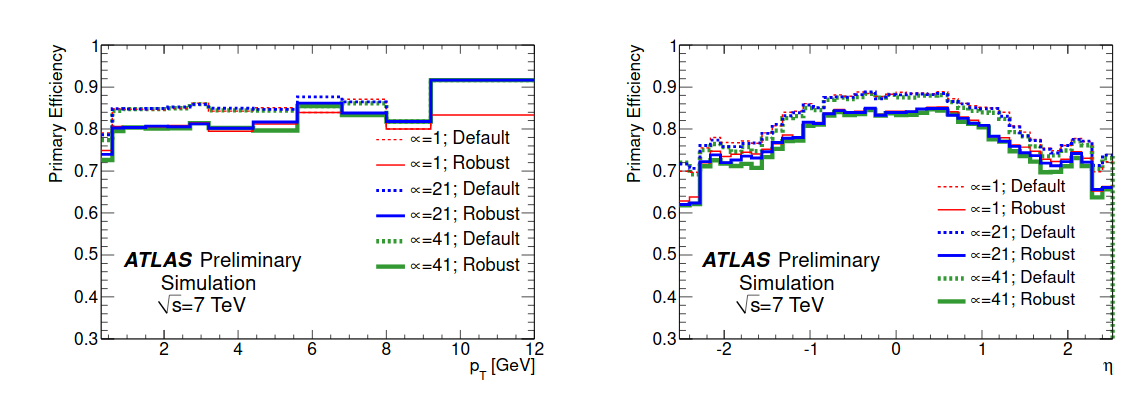
\includegraphics[width=0.9\textwidth]{Ch2/Img/Track_reco_eff.png}
    \caption{The primary track reconstruction efficiency in minimum bias Monte Carlo samples containing exactly one and on average 21 or 41 interactions. The distributions are shown for tracks passing the default(dashed) and robust (solid) requirements.}
    \label{fig:chap2:Objects:Trk:Eff}
\end{figure}
Primary vertices are reconstructed using an iterative vertex finding algorithm \cite{Vrtx_Eff}. Vertex seeds are obtained from the z-position at beam axis of the reconstructed tracks. An iterative $\chi^2$ fit constrained with the beam spot position is made using the seed and nearby tracks. Tracks are weighted depending on the $\chi^2$ to measure the compatibility with the fitted vertex \cite{chi2}. Tracks displaced by more than 7$\sigma$ from the vertex are used to seed a new vertex and the procedure is repeated until no additional vertices can be found. During reconstruction vertices are required to contain at least two tracks. The efficiency to reconstruct a vertex from a minimum bias interaction is shown in Figure \ref{fig:chap2:Objects:Vtx:Eff}. Vertices  are matched to interactions by calculating the sum of the weights of the tracks in a vertex matched to each interaction. 
\begin{figure}[ht]
    \centering
    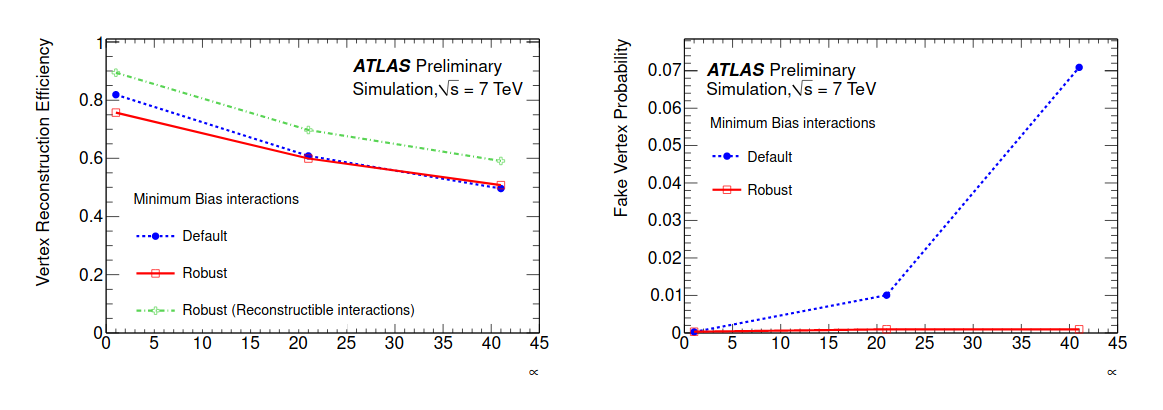
\includegraphics[width=0.9\textwidth]{Ch2/Img/Vtx_Reco_Eff.png}
    \caption{The vertex reconstruction efficiency ($left$) and fake probability ($right$) as a function of the aver-age number of interactions.}
    \label{fig:chap2:Objects:Vtx:Eff}
\end{figure}

\subsection{Electron and Photon reconstruction}
\label{chap2:Objects:Egamma}
Photons and Electrons are reconstructed in a similar way using the EM calorimeter (Section \ref{chap2:ATLAS:Calo:ECAL}). When these particles pass through the calorimeter dense medium, they start a showering process through cascading bremsstrahlung and electron pair production. Their shower are quite wide, therefore they deposit their energy in many calorimeter cells of each sampling. The electrical signal induced by electrons from ionised active material (LAr) is proportional to deposited energy in the active volume of the calorimeter and used to compute the cell energy. Note that, the cell energy includes both the electronic noise which is about 10 MeV in the strip and 30 MeV in the middle and back layers, and the $pile-up$ particles noise. The pile-up contributions can be either splitted into two components the $in-time$ pile-up which due to particles coming from the same bunch crossing, and the $out-of-time$ pile-up due to particles from previous bunch crossing. The total deposited energy is measured from the reconstructed EM clusters. To reconstruct the EM clusters, the EM calorimeter is divided into a grid of $N_\eta\times N\phi$ towers of size of the same middle layer granularity (0.025x0.025). Inside each of these elements, the energy of all cells in all longitudinal layers is summed into the tower energy. A window of fixed size 3×5 is moved across each element of the tower. If the window transverse energy \eT (defined as the sum of the transverse energy of the towers contained in the window) is a local maximum and is above a threshold (2.5 GeV), a cluster seed is formed. Then, if the reconstructed cluster can be associated with at least one reconstructed track, the candidate is classified as an electron. The described reconstruction algorithm until now is called $fixed-size$ \cite{Fixed_size_cluster}. \\
While, the reconstruction has been improved to use dynamic, variable-size clusters, called $super-clusters$ \cite{Egamma_Perf_run2}. This allows the recovery of low energy photons radiated due to bremsstrahlung interactions in the ID or electrons from photon conversions. In this scenario, the electron is defined as an object consisting of a super cluster and matched track. A converted photon is a cluster matched to a conversion vertex, and an unconverted photon is a cluster matched to neither an electron track or a conversion vertex. In contrast to the sliding window, the super-cluster selects clusters based on topologically connected calorimeter cells \cite{Topo_cluster}. Figure \ref{fig:chap2:Objetcs:Egamma:SC} shows an illustration of super-clusters. 
\begin{figure}[H]
    \centering
    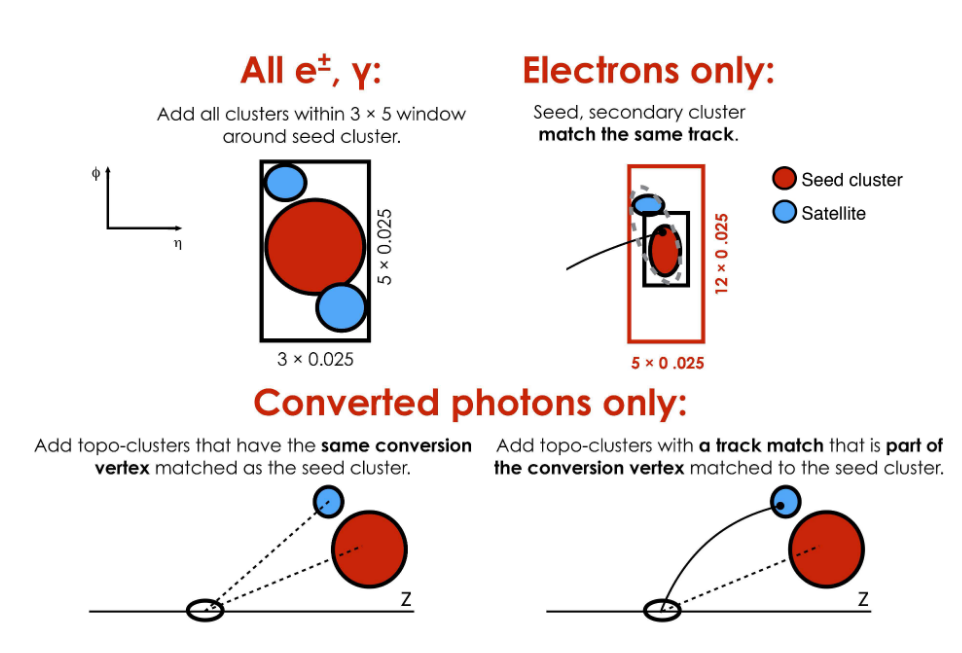
\includegraphics[width=0.7\textwidth]{Ch2/Img/Super_cluster.png}
    \caption{Diagram of the super clustering algorithm for electrons and photons. Seed clusters are shown in red, satellite clusters in blue.}
    \label{fig:chap2:Objetcs:Egamma:SC}
\end{figure}
The topo-cluster reconstruction starts from a cell with $|E_{cell}| > 4\sigma$, where $\sigma$ is the expected cell noise includes the known electronic noise and an estimation of the pile-up noises. Then successively, all neighbouring cells with $|E_{cell}| > 2\sigma$ are added. The absolute cell energy is used to avoid biasing the cluster energy upwards due to negative energy induced by the calorimeter noise. The list of reconstructed topo-clusters is sorted according to descending total energy. The topo-clusters are tested one by one for use as super-cluster. For an electron the topo-cluster is required to have a minimum $E_T$ of 1 GeV and matched to a track with at least four hits in the silicon detector \cite{GSF}, while for a photon the threshold is set to 1.5 GeV with no matched track or conversion vertex. For both, the electron and the photon case, to recover radiative losses, satellite clusters around that reconstructed cluster can be matched to the super-cluster. The seed clusters with their associated satellite clusters are called super-clusters. Tracks are matched to electron super clusters and conversion vertices to converted photon super clusters. The matching is performed in the same way that the matching to EM topo-clusters was performed, but using the super clusters instead. The reconstruction efficiency using super clusters for an electron is shown in Figure \ref{fig:chap2:Objects:Egamma:El_Eff}.
\begin{figure}[H]
    \centering
    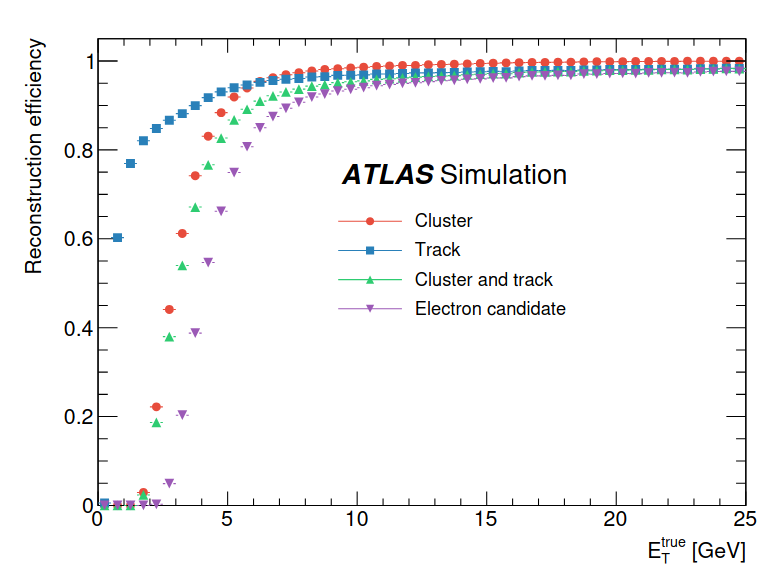
\includegraphics[width=0.5\textwidth]{Ch2/Img/Electron_Reco_Eff.png}
    \caption{The cluster, track, cluster and track, and electron reconstruction efficiencies as a function of the generated electron $E_T$.}
    \label{fig:chap2:Objects:Egamma:El_Eff}
\end{figure}
Figure \ref{fig:chap2:Objects:Egamma:Gamma:Conv:Reco:Eff} shows the reconstruction efficiency for converted photons as a function of the true $E_T$ of the simulated photon for the previous version of the reconstruction software (fixed-size) and the current version (dynamic-size). An important reason for using super clusters is the improved energy resolution that super clusters provide by collecting more of the deposited energy \textbf{ADD PLOT OF ENERGY RESOLUTION COMPARISON}.
\begin{figure}[H]
    \centering
    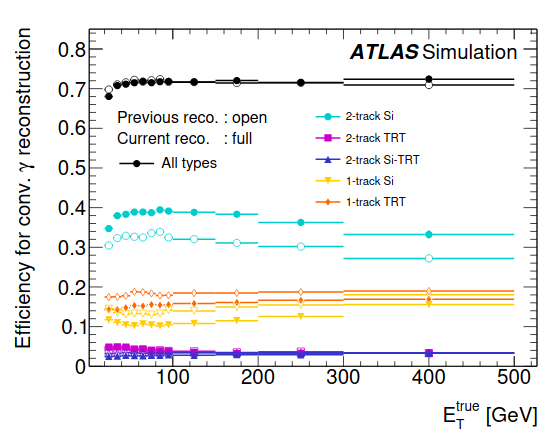
\includegraphics[width=0.5\textwidth]{Ch2/Img/Photon_conv_Reco_Eff.png}
    \caption{The converted photon reconstruction efficiency and contributions of the different conversion types as a function of $E^{true}_T$}
    \label{fig:chap2:Objects:Egamma:Gamma:Conv:Reco:Eff}
\end{figure}

Additionally, an ambiguity resolution is performed to remove a part of the overlap in case one object is reconstructed at the same time as electron and photon since electron and photon super clusters are built independently. However, in order to maintain a high reconstruction efficiency, a residual overlap is allowed, to allow physics analysis to define criteria based on their needs. Figure \ref{fig:chap2:Objects:Egamma:Ambg} shows the procedure used for ambiguity resolution. 
\begin{figure}[H]
    \centering
    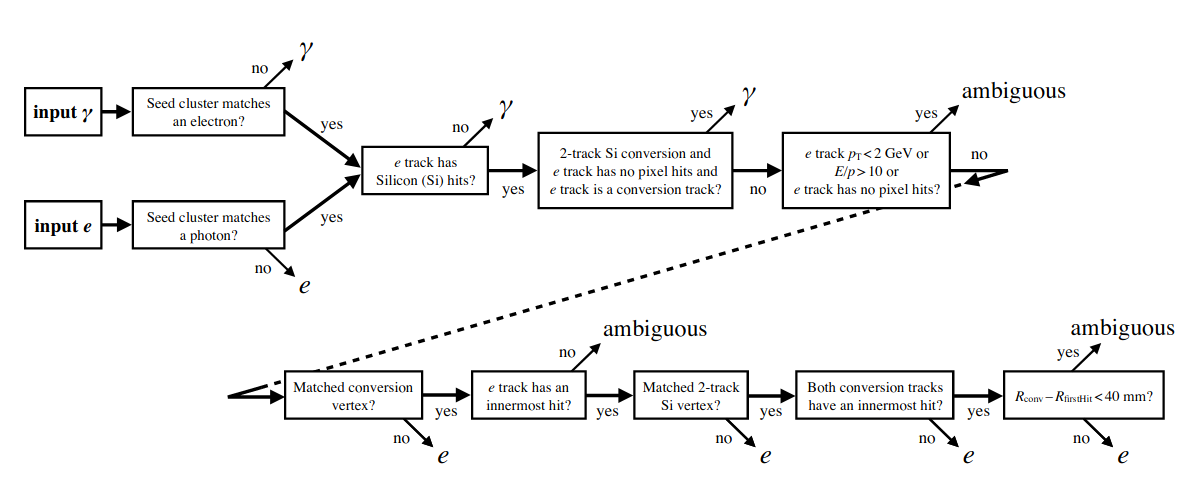
\includegraphics[width=0.8\textwidth]{Ch2/Img/Ambiguity.png}
    \caption{Flowchart showing the logic of the ambiguity resolution for particles initially reconstructed both as electrons and photons.}
    \label{fig:chap2:Objects:Egamma:Ambg}
\end{figure}

Most of LHC physics require the identification of prompt non-fake leptons and / or photons. Prompt particles are those not coming from a hadron or tau decay. Non-fake particles are those which type was properly reconstructed ($i.e.$ a non-fake reconstructed electron is a true electron, not another mis-identified particle). Their identification and separation can be obtained with several selection criteria and algorithms. The identification for the reconstructed electrons and photons is finally based on the reconstructed super-cluster objects. A set of discriminating variables are calculated for the identification using cells in the fixed-size window. A list is given in Table \ref{tab:chap2:Objects:Egamma:SS} long with an indication if they are used for electron or photon identification. The prompt and non-fake leptons/photons are usually isolated, without much activity around them. It is therefore important to define a proper "isolation criteria" to reduce the contamination from non-prompt and fake objects. Electron isolation and identification are described in Sections \ref{chap2:Objects:Egamma:EIso} and \ref{chap2:Objects:Egamma:EID} respectively, while Chapter \ref{gamma} is dedicated to photon proprieties.
\begin{table}[tp]
    
    \caption{Discriminating variables used for electron and photon
    identification. The usage column indicates if the variables are
    used for the identification of electrons, photons, or both. \cite{Egamma_Perf_run2}.}
   \def\arraystretch{1.3}
   \centering 
   \footnotesize
  \begin{tabular}{
  l
  >{\RaggedRight}p{0.55\textwidth}
  lc}
  \hline 
  \hline
  Category & Description & Name & Usage \\
  \hline 
  \hline
  Hadronic leakage
  & Ratio of $E_\mathrm{T}$ in the first layer of the hadronic calorimeter to $E_\mathrm{T}$ of the
    EM cluster (used over the ranges $|\eta|<0.8$ and $|\eta|>1.37$)  & $\Rhadone$ & $e/\gamma$  \\
  & Ratio of $E_\mathrm{T}$ in the hadronic calorimeter to $E_\mathrm{T}$ of the EM cluster
    (used over the range $0.8<|\eta|<1.37$)  & $\Rhad$  & $e/\gamma$ \\

  EM third layer
  & Ratio of the energy in the third layer to the total energy in the EM calorimeter & $\fIII$ & $e$ \\  

  EM second layer
  & Ratio of the sum of the energies of
  the cells contained in a $3\times7$ ($\eta\times\phi$)
  rectangle (measured in cell units)  to the sum of
  the cell energies in a $7\times7$ rectangle, both centred around the
  most energetic cell & $\Reta$ & $e/\gamma$ \\
  & Lateral shower width, $\sqrt{(\Sigma E_i \eta_i^2)/(\Sigma E_i)
    -((\Sigma E_i\eta_i)/(\Sigma E_i))^2}$, where $E_i$ is the energy
    and $\eta_i$ is the pseudorapidity of cell $i$ and the sum is calculated within a window of $3\times5$ cells
     & $\wetatwo$ & $e/\gamma$ \\
  & Ratio of the sum of the energies of
  the cells contained in a $3\times3$ ($\eta\times\phi$)
  rectangle (measured in cell units) to the sum of
  the cell energies in a $3\times7$ rectangle, both centred around the
  most energetic cell  & $\Rphi$ & $e/\gamma$ \\

  EM first layer
  & Total lateral shower width, $\sqrt{(\Sigma E_i
    (i-i_\mathrm{max})^2)/(\Sigma E_i)}$, where $i$ runs over all
    cells in a window of $\Delta\eta \approx 0.0625$ and
    $i_{\textrm{max}}$ is the index of the highest-energy cell
     & $\wtot$ & $e/\gamma$ \\
  & Lateral shower width,
    $\sqrt{(\Sigma E_i (i - i_{\textrm{max}})^2)/(\Sigma E_i)}$,
    where $i$ runs over all cells in a window of 3 cells around the
    highest-energy cell & $\wthree$ & $\gamma$ \\
  & Energy fraction outside core of three central cells, within seven cells   & $\Fside$ & $\gamma$ \\
  & Difference between the energy of the cell associated with the
    second maximum, and the energy reconstructed
    in the cell with the smallest value found between the first and
    second maxima  & $\DeltaE$ & $\gamma$ \\
  & Ratio of the energy difference between the maximum energy deposit and the energy deposit in a secondary maximum in the cluster to the sum of these energies   & $\Eratio$ & $e/\gamma$ \\
  & Ratio of the energy measured in the first layer of the electromagnetic calorimeter to the total energy of the
    EM cluster & $\fI$ & $e/\gamma$ \\

    Track conditions
           & Number of hits in the innermost pixel layer &   $n_\mathrm{innermost}$ & $e$ \\
           & Number of hits in the pixel detector        &    $n_\mathrm{Pixel}$ & $e$ \\
           & Total number of hits in the pixel and SCT detectors  &   $n_{\mathrm{Si}}$  & $e$ \\
           & Transverse impact parameter relative to the beam-line &  \trackdO  & $e$ \\
           & Significance of transverse impact parameter defined as
              the ratio of \trackdO to its uncertainty &  $|\dOSignificance|$  & $e$  \\
           &  Momentum lost by the track between the perigee and the last measurement point divided by
             the momentum at perigee& \deltapoverp & $e$ \\
           & Likelihood probability based on transition radiation in the TRT &   \TRTPID & $e$  \\
    Track--cluster matching
           & $\Delta\eta$ between the cluster position in the first layer 
             of the EM calorimeter and the extrapolated track &   \deltaeta & $e$  \\
           & $\Delta\phi$ between the cluster position in the second layer
             of the EM calorimeter and the momentum-rescaled track,
             extrapolated from the perigee, times the charge $q$ & \deltaphires & $e$  \\
            &  Ratio of the cluster energy to the measured track momentum  &       $E/p$   &  $e$ \\
  \hline 
  \hline
  \end{tabular}
  \label{tab:chap2:Objects:Egamma:SS}
\end{table}

\subsubsection{Electron and Photon calibration}
\label{chap2:Objects:Egamma:Cal}
After the electron and photon super clusters are built, an initial energy calibration and position correction is applied to them \cite{Egamma_Calibration}. A complex chain with several successive calibration steps is used to calibrate the electron and photon energies based on simulation and well known reference processes. A schematic overview of the whole calibration chain is shown in Figure \ref{fig:chap2:Objects:Egamma:Cal}.
\begin{figure}[H]
    \centering
    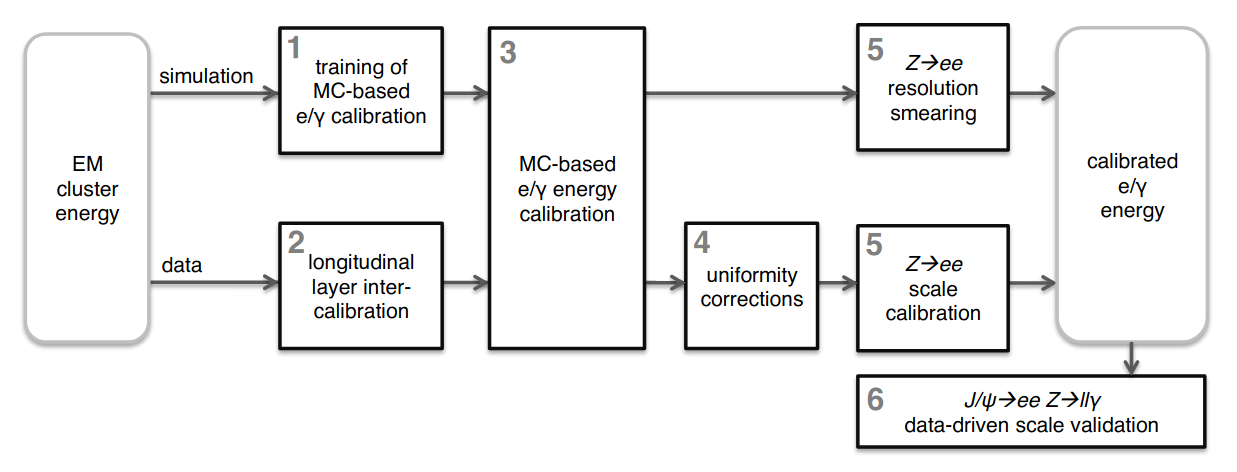
\includegraphics[width=0.6\textwidth]{Ch2/Img/Calibration_Chain.png}
    \caption{Schematic overview of the calibration chain for the electron and photon energies \cite{Egamma_Calib_run1}.}
    \label{fig:chap2:Objects:Egamma:Cal}
\end{figure}
\begin{enumerate}
    \item Multivariate regression algorithm is trained on the properties of the shower development in the EM calorimeter to optimize the energy resolution and to minimize the impact of material in front of the calorimeter. The algorithm used in this step is the Boosted Decision Trees (BDTs) tuned in intervals of $|\eta|$ and $E_T$ on samples of simulated single particles without pile-up, separately for electrons, converted and unconverted photons. 
    \item An inter-layer correction is applied to the relative energy response in data to match the relative response in MC in different calorimeter layers. The inter-layer calibration is independent from the material upstream of the calorimeter.
    \item The BDTs correction is applied to both data and MC. This step performs the main correction of the absolute energy scale and improves significantly the energy resolution.
    \item The non simulated detector non-uniformities are therefore corrected in data. Correcting the effects of energy loss between the barrel calorimeter modules and the high-voltage inhomogeneities.
    \item Scale factors are applied to the energy in data to correct for the residual miscalibration between data and MC using $Z\rightarrow e^+e^-$ events.
    \item The validity of the calibration is cross checked from data using different processes. For the low energy range $J/\Psi\rightarrow e^+e^-$ events are used. The calibration for photons is cross-checked using radiative $Z\rightarrow l^+l^-\gamma$ ($l=e,\mu$) decays.
\end{enumerate}
\subsubsection{Electron Isolation}
\label{chap2:Objects:Egamma:EIso}
The activity near leptons and photons can be quantified from the tracks of nearby charged particles or from energy deposits in the calorimeters, leading to tow classes of isolation variables calorimeter based isolation $E^{coneXX}_{T}$ and track-based $p_T^{coneXX}$ \cite{Electron_Reco_Id_Run1}. The corrected $E^{coneXX}_{T}$ is computed as the sum of the transverse energies of topo-clusters inside a cone of $\Delta R = \frac{XX}{100}$ around the reconstructed electrons, this is illustrated in Figure \ref{fig:chap2:Objects:Egamma:EIso:Schema}, after subtraction of the energy deposited by the electrons, pileup and underlying event \cite{PileUp_IsoExtract}. The $p_T^{coneXX}$ is computed by summing the transverse momentum of selected tracks of \pT $>$ 1 GeV and $|\eta|<$ 2.5, within a cone centred around the electron track. Tracks matched to the electron are excluded. In a high-momentum heavy particles decay, the electron is produced very close to other decay products, for this reason an isolation $p_T^{varconeXX}$ with a variable cone size $\Delta R^{XX}$ is defined the cone size shrinks for larger \pT electrons:
\begin{equation}
    \Delta R^{XX} = min(\frac{10}{p_T[GeV]}, \frac{XX}{100}).
\end{equation}
\begin{figure}[ht]
    \centering
    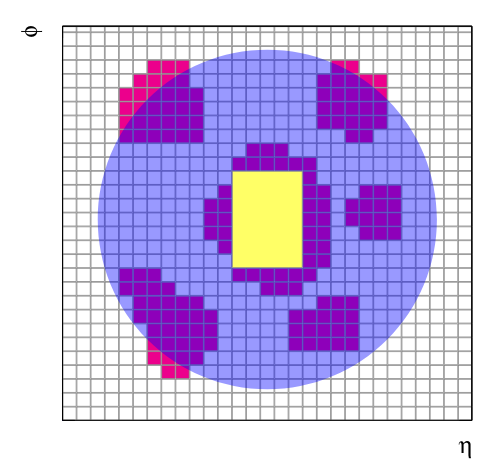
\includegraphics[width=0.5\textwidth]{Ch2/Img/Iso_Schema.png}
    \caption{Schema of the calorimeter isolation method: the grid represents the second-layer calorimeter cells in the $\eta$ and $\phi$ directions. The candidate electron is located in the centre of the purple circle representing the isolation cone. All topological clusters, represented in red, for which the barycentres fall within the isolation cone are included in the computation of the isolation variable. The 5x7 cells represented by the yellow rectangle correspond to the subtracted cells in the core subtraction method.}
    \label{fig:chap2:Objects:Egamma:EIso:Schema}
\end{figure}
Based on these variables, three different selections criteria, called working points (WPs), are implemented. The working points can be defined in two different ways, either targeting a fixed value of efficiency or with fixed cuts on the isolation variables. Table \ref{tab:chap2:Objects:Egamma:EIso:WPs} lists the different electron-isolation WPs used in ATLAS.
\begin{table}[H]
    \centering
    \begin{tabular}{ccc}
    \hline \hline
        WP & Calorimeter-based isolation & Track-based isolation \\ \hline 
        HighPtCaloOnly & $E^{cone20}_T < max(0.015\times p_T, 3.5 GeV)$ & - \\
        Loose & $E^{cone20}_T/p_T < 0.2$ & $p^{varcone20}_T/p_T < 0.15$ \\
        Tight & $E^{cone20}_T/p_T < 0.06$ & $p^{varcone20}_T/p_T < 0.06$ \\ \hline \hline
    \end{tabular}
    \caption{Definition of the electron isolation working points.}
    \label{tab:chap2:Objects:Egamma:EIso:WPs}
\end{table}
An additional WP named Gradient is designed to give an efficiency of 90\% at \pT = 25 GeV and 99\% at 60 GeV, uniform in $\eta$. Figure \ref{fig:chap2:Objects:Egamma:EIso:Eff} shows the electron isolation efficiency in data recorded in 2017 as a function of electron \eT \cite{Egamma_Perf_2017}. The method used to compute the electron isolation efficiency and the associated uncertainties are described in Ref. \cite{Electron_Reco_Id_Run1}. The jump observed in Gradient efficiency at 15 GeV is due to the fact the the isolation efficiency is process dependent: the Gradient cut maps is optimized with $J/Psi\rightarrow e^+e^-$ events below 15 GeV, while the efficiency measurement is performed with $Z\rightarrow e^+e^-$.
\begin{figure}[ht]
    \centering
    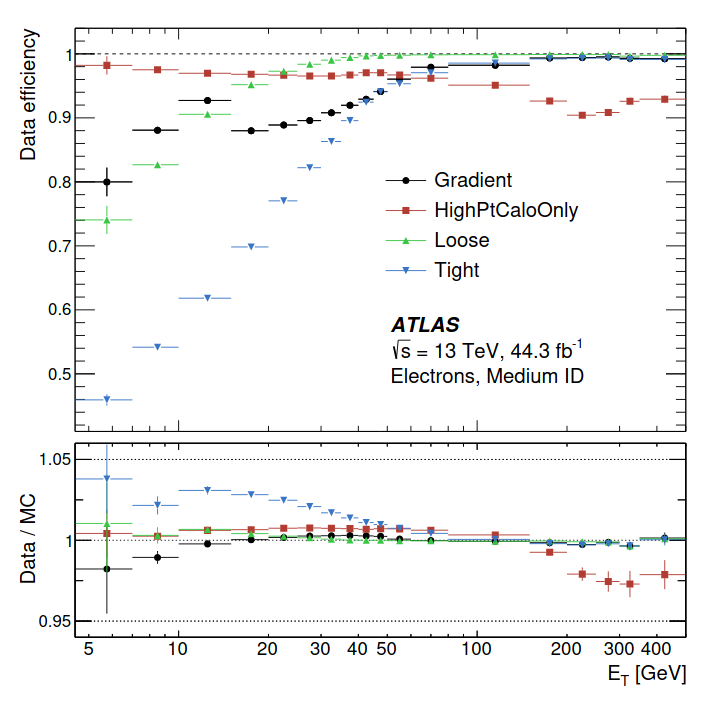
\includegraphics[width=0.5\textwidth]{Ch2/Img/Electron_Iso_Eff.png}
    \caption{Efficiency of the different isolation working points for electrons from inclusive $Z\rightarrow e^+e^-$ events as a function of the electron \eT. The lower panel shows the ratio of the efficiencies measured in data and in MC simulations \cite{Egamma_Perf_2017}.}
    \label{fig:chap2:Objects:Egamma:EIso:Eff}
\end{figure}
\subsubsection{Electron Identification}
\label{chap2:Objects:Egamma:EID}
The identification of prompt electrons relies on a likelihood (LH) discriminant constructed from quantities measured in the different sub-detectors and listed in Table \ref{tab:chap2:Objects:Egamma:SS}. The electron LH is based on the products of the probability density functions (PDFs) for signal $L_S$, and for background $L_B$. The PDFs are created by smoothing histograms of the n discriminating variables with an adaptive kernel density estimator (KDE) \cite{KDE} as implemented in TMVA \cite{TMVA} in 9 bins in $|\eta|$ and 7 bins of \eT:
\begin{equation}
    L_{S(B)}(\textbf{x}) = \displaystyle\prod_{i=1}^{n} P_{S(B),i}(x_i),
\end{equation}
where \textbf{x} is the vector of the various variables. For each electron candidate, a discriminant $d_L$ is formed using an inverse sigmoid function transformation:
\begin{equation}
    d_L = -\frac{1}{\tau}ln(\frac{L_S+L_B}{L_S} - 1),
\end{equation}
where $\tau$ is fixed to 15 \cite{TMVA}. Figure shows the an example of the distribution of the transformed discriminant for prompt electrons and for non-prompt one. This distribution illustrates the effective separation between signal and background encapsulated in this single quantity.
\begin{figure}[H]
    \centering
    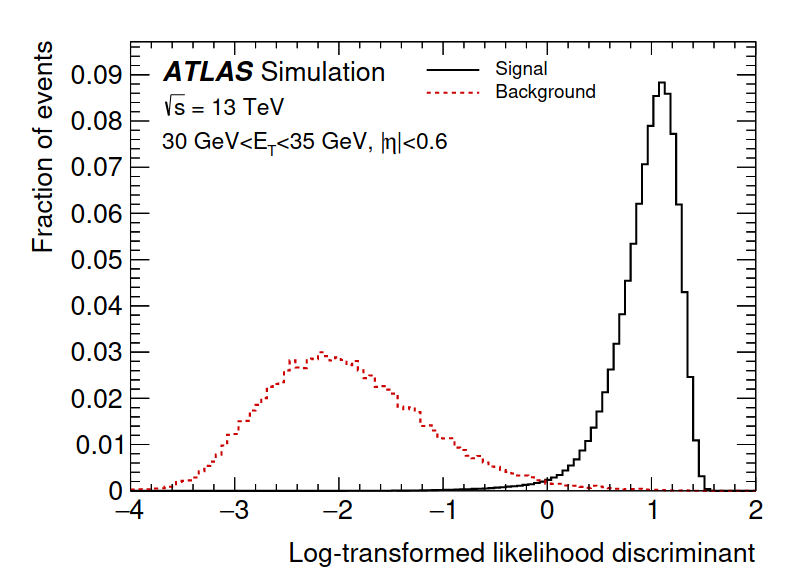
\includegraphics[width=0.5\textwidth]{Ch2/Img/Electron_LH.png}
    \caption{The transformed LH-based identification discriminant $d_L$ for reconstructed electron candidates with good quality tracks with 30 $<E_T<$ 35 GeV and $|\eta|<$ 0.6 \cite{Electron_ID_2016}.}
    \label{fig:chap2:Objects:Egamma:EID:LH}
\end{figure}
For physics purposes three WPs are defined. These operating points are referred to as Loose, Medium, and Tight. The efficiency for identifying a prompt election with \eT = 40 GeV are 93\%, 88\% and 80\% for the Loose, Medium and Tight. Figure \ref{fig:chap2:Objects:Egamma:EID:Eff} shows the resulting efficiencies in data \cite{Egamma_Perf_run2}. 
\begin{figure}[H]
    \centering
    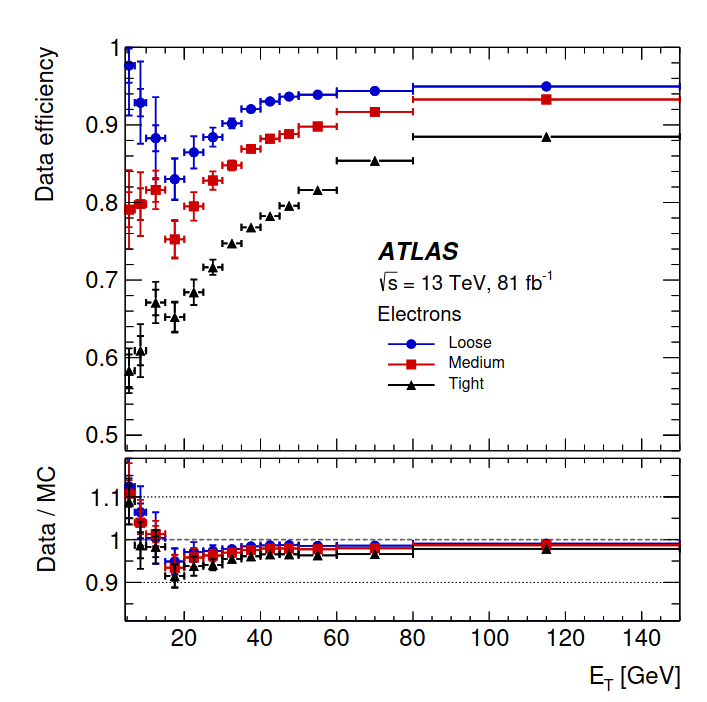
\includegraphics[width=0.5\textwidth]{Ch2/Img/Electron_ID_Eff.png}
    \caption{The electron identification efficiency in $Z\rightarrow e^+e^-$ events in data as a function of \eT for the Loose, Medium and Tight operating points.}
    \label{fig:chap2:Objects:Egamma:EID:Eff}
\end{figure}

\subsection{Muon reconstruction and identification}
\label{chap2:Objects:Muon}
\subsubsection{Muon reconstruction}
\label{chap2:Objects:Muon:Reco}
Muons are the only charged particles leaving the calorimeter system. Muon reconstruction is performed in two sub-detectors independently. Firstly, the muon tracks are reconstructed in the ID like any track as described in Section \ref{chap2:Objects:Trk}. Then, the ID reconstruction is combined with the muon reconstruction in MS sub-detector to perform the muon object used in physics analysis. In the MS, the muons are triggered in RPC/TGC if at least one hut exists, defining the region of activity (ROA). All the muon chambers intersecting with the ROA are then selected as muon track candidates. The MDT segments are reconstructed by performing a straight-line fit (the bending of muons $>$ few GeV is sufficiently small) to the hits found in each layer \cite{hough}. The fitted segments are required to point loosely towards the IP, in order to reject background events and random hit combinations. Muon track candidates are then built by extrapolation each of these segments to the other. At least two matching segments  using their relative positions and angles are required to build a track, except in the barrel–endcap transition region where a single high-quality segment can be used. \\
The combined reconstruction is performed according to various algorithms based on the provided information by sub-detectors \cite{Muon_Reco_2014_algo,Muon_Reco_2016_algo}: 
\begin{itemize}
    \item Combined (CB) muon: the combined muon is formed with a global refit that used the hits from both the ID and MS sub-detectors. The reconstruction is done following two complementary approaches, the outside-in in which the the reconstructed track in the MS are extrapolated inward and match to an ID track, and the inside-out reconstruction, in which ID tracks are extrapolated outward and matched to MS tracks. 
    \item Segment-tagged (ST) muon: ST muons are used when muons cross only one layer MS chamber, either because of their low \pT or because of MS acceptance. 
    \item Calorimeter-tagged (CT) muon: reconstructed track with an energy deposit in the calorimeter compatible with a minimum-ionizing particle is identified as CT muon. 
    \item Extrapolated (ME) muon: ME muons are reconstructed based only on the MS track and a loose requirement on compatibility with originating from the IP. 
\end{itemize}
Overlaps between different muon types are resolved with preference to CB, ST and CT muons respectively before producing the collection of muons used in physics analyses.

\subsubsection{Muon identification}
\label{chap2:Objects:Muon:ID}
In order to suppress muons coming from background, mainly pion and kaon decays, and select prompt muons, a muon identification is performed. Muon identification uses several variables, for CB tracks, the variables used are: 
\begin{itemize}
    \item $q/p \ significance$ defined as : 
    \begin{equation}
        q / p \ significance=\frac{\left|q / p_{\mathrm{ID}}-q / p_{\mathrm{MS}}\right|}{\sqrt{\sigma^{2}\left(q / p_{\mathrm{ID}}\right)+\sigma^{2}\left(q / p_{\mathrm{MS}}\right)}},
    \end{equation}
    where $q/p_{ID}$ and $q/p_{MS}$ are the measurements in the ID ans MS of the ratio of the charge $q$ to the momentum $p$ of the muon, expressed at the IP and $\sigma$ is the corresponding uncertainties. 
    \item $\rho'$, defined as the absolute value of the difference between the transverse momentum measurements in the ID ans MS divided by the \pT of the combined track.
    \item Normalised $\chi^2$ of the combined track fit. 
\end{itemize}

Four muon identification WPs are provided to address specific needs of different physics analysis:
\begin{itemize}
    \item $Loose$ : identification criteria are designed to maximise the reconstruction efficiency while providing good-quality muon tracks. They are specifically optimised for reconstructing Higgs boson candidates in the four-lepton final state \cite{Higgs_4leptons}.
    \item $Medium$ : identification criteria provide the default selection for muons in ATLAS. This selection minimises the systematic uncertainties associated with muon reconstruction and calibration. Only CB and ME tracks are used. About 0.5\% of Medium muon originate from the inside-out reconstruction strategy, in the central region. 
    \item $Tight$ : muons are selected to maximise the purity of muons at the cost of some efficiency. Only CB muons with hits in at least two stations of the MS and satisfying the $Medium$ selection criteria are considered.
    \item $High-p_T$ : selection  aims  to  maximise the momentum resolution  for  tracks  with transverse momentum above  100 GeV. The  selection is optimised  for  searches  for  high-mass Z' and W' resonances \cite{W,dilepton}. CB muons passing the $Medium$ selection  and having at least three hits in three MS stations are selected.
\end{itemize}
Figure \ref{fig:chap2:Objects:Muon:ID:Eff} shows the muon reconstruction and identification efficiency for $Loose$, $Medium$ and $Tight$ muons as measured in $J/\Psi\rightarrow\mu\mu$. 
\begin{figure}[H]
    \centering
    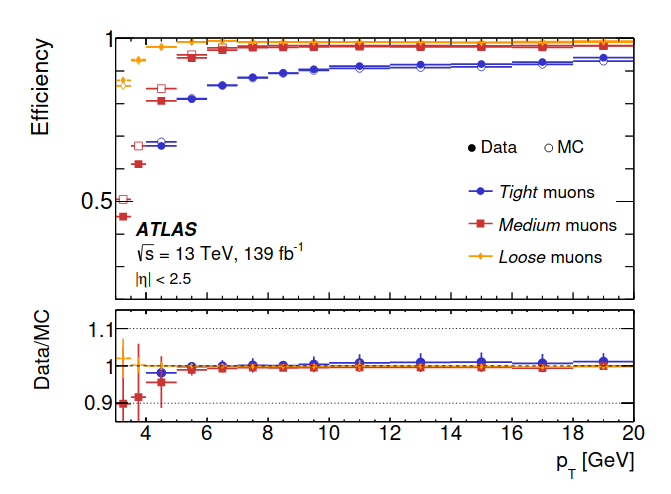
\includegraphics[width=0.5\textwidth]{Ch2/Img/Muon_ID_Eff.png}
    \caption{Muon reconstruction and identification efficiencies for the $Loose$, $Medium$ and $Tight$ criteria as function of \pT. The panel at the bottom shows the ratio of the measured to predicted efficiencies, with statistical and systematic uncertainties.}
    \label{fig:chap2:Objects:Muon:ID:Eff}
\end{figure}

\subsection{Jet reconstruction}
\label{chap2:Objects:Jet}
Jets are made of a large number of partons coming from the initial quark or gluon hadronisation, appearing in the detector as a collimated shower. Many jets reconstruction algorithms exits, only two approaches are of interest for the work presented in this thesis. The first approach is based exclusively on electromagnetic and hadronic topological clusters, so-called EMTopo jets. The second approach uses both tracking and calorimetric information through a Particle Flow algorithm to build PFlow jets \cite{Jet_Perf_Run2}. Jets are identified using the anti-$k_t$ algorithm \cite{Anti-Kt}, with a distance parameter R=0.4. Jets reconstruction and calibration will be discussed in Chapter \ref{Jet}. 

\subsection{Missing transverse energy}
\label{chap2:Objects:MET}
Neutrinos and other BSM particles interact extremely weakly with matter, making the hard to detect and they cannot be observed directly as hadrons, electrons or muons discussed before. Their energy is reconstructed as missing transverse energy (MET). Thanks to momentum conservation, the transverse momentum of all particles generated in a collision should sum up to zero, since the original transverse momentum of the partons is negligible. MET is defined as the sum of the transverse energy momenta of all reconstructed objects $i$: 
\begin{equation}
    \vec{E}_{T}^{m i s s}=-\sum_{i} \vec{p}_{T}^{i}
\end{equation}
